\documentclass{article}


\newcommand{\dir}{../../latex}
\input{\dir/include.tex}
\load{recommended}

\setup{Algorithms and Probability}

\begin{document}
\startDocument
\usetcolorboxes
\setcounter{numberingConfig}{3}

\vspace{2cm}
\begin{Huge}
    \begin{align*}
          & \Pr[X|Y] \geq \Pr[X|\overline{Y}] \\
        X & := \text{I pass the exam}         \\
        Y & := \text{I read this summary}
    \end{align*}
\end{Huge}


\vspace{4cm}
\begin{center}
    \begin{Large}
        ``\textit{Dieses Algorithmus mapped $E$ nach $E$ Strich}''
    \end{Large}

    \hspace{3cm} - Rasmus Kyng, 2025
\end{center}

\vspace{3cm}
\begin{center}
    FS2025, ETHZ\\[0.2cm]
    \begin{Large}
        Summary of the Script and Lectures
    \end{Large}\\[0.2cm]
\end{center}




\newpage
\printtoc{ForestGreen}

% Graph algorithms
\newsection
\section{Introduction}

\subsection{Sufficiency \& Necessity}
\begin{definition}[]{Sufficiency}
    A condition $P$ is called \textit{sufficient} for $Q$ if knowing $P$ is true is enough evidence to conclude that $Q$ is true.

    This is equivalent to saying $Q \Rightarrow P$.
\end{definition}

\begin{definition}[]{Necessity}
    A condition $P$ is called \textit{necessary} for $Q$ if $Q$ cannot occur unless $P$ is true, but doesn't imply that $Q$ is true, only that it is false if $P$ is false.

    This is equivalent to saying $P \Rightarrow Q$
\end{definition}

\subsection{Asymptotic Growth}
$f$ grows asymptotically slower than $g$ if $\displaystyle\lim_{m \rightarrow \infty} \frac{f(m)}{g(m)} = 0$.
We can remark that $f$ is upper-bounded by $g$, thus $f \leq \tco{g}$ and we can say $g$ is lower bounded by $f$, thus $g \geq \tcl{f}$.
If two functions grow equally fast asymptotically, $\tct{f} = g$


\subsection{Runtime evaluation}
Identify the basic operations (usually given by the task), then count how often they are called and express that as a function in $n$.
It is easier to note that in sum notation, then simplify that sum notation into a formula not containing any summation symbols.


% ────────────────────────────────────────────────────────────────────
\subsection{Tips for Converting Summation Notation into Summation-Free Notation}

\subsubsection{Identify the Pattern:}
\begin{itemize}
    \item Examine the summand.
    \item Look for patterns related to the index variable (usually $i$, $j$, etc.). Is it a linear function, a power of $i$, a combination?
\end{itemize}


\subsubsection{Arithmetic Series Formula}
If the summand is a simple arithmetic progression (e.g., $a + bi$ where $a$ and $b$ are constants), use the formula:
\[
    \sum_{i=m}^{n} (a + bi) = (n - m + 1)\left(a + b\frac{m + n}{2}\right)
\]


\subsubsection{Power Rule for Sums}
\begin{itemize}
    \item For sums involving powers of $i$, you can use the following pattern:
          \[
              \sum_{i=1}^{n} i^k = \frac{n^{k+1}}{k+1}
          \]
    \item Remember that this rule only applies when the index starts at 1.
\end{itemize}


\subsubsection{Telescoping Series}
Look for terms in consecutive elements of the summand that cancel out, leaving a simpler expression after expanding. This is particularly helpful for fractions and ratios.


\subsubsection{Geometric Series Formula}
For sums involving constant ratios (e.g., $a \cdot r^i$ where $r$ is the common ratio), use:
\[
    \sum_{i=0}^{n} a \cdot r^i = a \frac{1 - r^{n+1}}{1-r}
\]


\subsubsection{Gaussian Formula}
If $S$ is an arithmetic series with $n$ terms, then $S = \frac{n}{2} * (a + 1)$


\subsubsection{Examples}
The only other way (other than learning these tips) in which you are going to get better at this is by parctising.
Work through examples, starting with simpler ones and moving towards more complex expressions.


\fhlc{Aquamarine}{Example:}

Let's convert the summation: $\sum_{i=1}^{5} i$

\begin{enumerate}
    \item \textbf{Pattern:} The summand is simply $i$, which represents a linear arithmetic progression.

    \item \textbf{Arithmetic Series Formula:} Applying the formula with $a = 1$, $b = 1$, $m = 1$, and $n = 5$:
          \[
              \sum_{i=1}^{5} i = (5 - 1 + 1)\left(1 + 1 \cdot \frac{1 + 5}{2}\right) = 5 \cdot 3 = 15
          \]
\end{enumerate}

Therefore, the summation evaluates to $15$.

\subsection{Specific examples}
\begin{align*}
    \frac{n}{\log(n)} \geq \Omega(\sqrt{n}) \Leftrightarrow \sqrt{n} \leq \tco{\frac{n}{\log(n)}}
\end{align*}

\setcounter{subsection}{3}
\subsection{Connectivity}
\setcounter{all}{23}
% Page 37
\begin{definition}[]{$k$-Connected graph}
    A graph $G = (V, E)$ is called $k$\textit{-connected} if $|V| \geq k + 1$ and for all subsets $X \subseteq V$ with $|X| < k$ we have that the graph $G[V\backslash X]$ is connected
\end{definition}
If $G[V\backslash X]$ is \bi{not} connected, we call it a \textit{(vertex)-separator}.

A $k$-connected graph is also $k - 1$ connected, etc

\begin{definition}[]{$k$-edge-connected}
    A graph $G = (V, E)$ is called $k$\textit{-edge-connected} if for all subsets $X \subseteq E$ with $|X| < k$ we have: The graph $(V, E\backslash X)$ is connected
\end{definition}
We also have \textit{edge-separators}, defined analogously to above, i.e. the set $X$ above is called a $u$-$v$-edge-separator if by removing it from the graph, $u$ and $v$ no longer lay in the same connected component.

If a graph is $k$-edge-connected, it is also $k - 1$-edge-connected, etc


\begin{theorem}[]{Menger's theorem}
    Let $G = (V, E)$ be a graph and $u \neq v \in V$. Then we have
    \begin{enumerate}
        \item Every $u$-$v$-vertex-separator has size at least $k \Leftrightarrow$ Exist at least $k$ internally vertex-disjoint $u$-$v$-paths
        \item Every $u$-$v$-edge-separator has size at least $k \Leftrightarrow$ Exist at least $k$ edge-disjoint $u$-$v$-paths
    \end{enumerate}
\end{theorem}


\newpage
\subsubsection{Articulation points}
If a graph is connected, but not $2$-connected, there exists at least one vertex $v$ for which, if removed, the graph is not connected, called \textit{articulation points}. Using a modified DFS, we can find these vertices. Instead of just setting a flag for each vertex we visit, we set a number indicating the order in which the vertices were visited. The first vertex we visit, for instance, gets number $1$.

We also add another value, which we call \verb|low[v]| $:=$ the smallest DFS-number that can be reached from $v$ using a path of arbitrarily many edges of the DFS-tree and at most one residual edge.

We also have (where $s$ is the start / source vertex and $E(T)$ is the edge set of the DFS-tree):

$v$ is an articulation point $\Leftrightarrow$ ($v = s$ and $s$ has degree at least $2$ in $T$) or ($v \neq s$ and there exists $w \in V$ with $\{(v, w)\} \in E(T)$ and $\verb|low[w]| \geq \verb|dfs[v]|$)


\begin{algorithm}
    \caption{\textsc{FindArticulationPoints}($G, s$)}
    \begin{algorithmic}[1]
        \State $\forall v \in V$: \texttt{dfs[v]}$\gets 0$ \Comment{Stores dfs number for vertex $v$ and also flag for visit}
        \State $\forall v \in V$: \texttt{low[v]}$\gets 0$ \Comment{Stores low point for vertex $v$}
        \State $\forall v \in V$: \texttt{isArticulationPoint[v]}$\gets \texttt{false}$ \Comment{Indicates if vertex $v$ is articulation point}
        \State \texttt{num} $\gets 0$
        \State $T \gets \emptyset$ \Comment{Depth-First-Search Tree}
        \State \Call{DFS-Visit}{$G, s$}
        \If{$s$ has degree at least two in $T$} \Comment{Start vertex classification could be incorrect from \textsc{DFS-Visit}}
            \State $\texttt{isArticulationPoint[s]} \gets \texttt{true}$
        \Else
            \State $\texttt{isArticulationPoint[s]} \gets \texttt{false}$
        \EndIf
        \Procedure{DFS-Visit}{$G, v$}
            \State \texttt{num} $\gets$ \texttt{num} $+ 1$
            \State \texttt{dfs[v]} $\gets$ \texttt{num}
            \State \texttt{low[v]} $\gets$ \texttt{dfs[v]}
            \For{\textbf{all} $\{v, w\} \in E$}
                \If{\texttt{dfs[w]} = 0}
                    \State $T \gets T \cup \{\{v, w\}\}$
                    \State $\texttt{val} \gets$ \Call{DFS-Visit}{$G, w$}
                    \If{$\texttt{val} \geq \texttt{dfs[v]}$} \Comment{Check articulation point condition}
                        \State $\texttt{isArticulationPoint[v]} \gets \texttt{true}$
                    \EndIf
                    \State $\texttt{low[v]} \gets \min \{\texttt{low[v]}, \texttt{val}\}$
                \ElsIf{$\texttt{dfs[w]} \neq 0$ \textbf{and} $\{v, w\} \notin T$} \Comment{Update low if already visited}
                    \State $\texttt{low[v]} \gets \min \{\texttt{low[v]}, \texttt{dfs[w]}\}$
                \EndIf
            \EndFor
            \State \Return \texttt{low[v]}
        \EndProcedure
    \end{algorithmic}
\end{algorithm}

\stepcounter{all}
\begin{theorem}[]{Articulation points Computation}
    For a connected graph $G = (V, E)$ that is stored using an adjacency list, we can compute all articulation points in \tco{|E|}
\end{theorem}


\newpage
\subsubsection{Bridges}
While articulation points show that a graph is not $2$-connected, bridges shows that a graph isn't $2$-edge-connected.
In other words, they are certificates for the graph \textit{not} being $2$-edge-connected or more formally:

\begin{center}
    \fbox{
        \textit{
            An edge $e \in E$ in a connected graph $G = (V, E)$ is called a bridge if the graph $(V, E\backslash \{e\})$ is not connected.
        }
    }
\end{center}

From the definition of bridges we immediately have that a spanning tree has to contain all bridges of a graph, and we can also state that only edges of a Depth-First-Search-Tree are possible candidates for a bridge.

The idea now is that every vertex contained in a bridge is either an articulation point or has degree $1$ in $G$. Or more formally:

\begin{center}
    \fbox{
        \textit{
            A directed edge $(v, w)$ of Depth-First-Search-Tree $T$ is a bridge if and only if $\texttt{low[w]} > \texttt{dfs[v]}$
        }
    }
\end{center}

\begin{theorem}[]{Bridges Computation}
    For a connected graph $G = (V, E)$ that is stored using an adjacency list, we can compute all bridges and articulation points in \tco{|E|}
\end{theorem}

\subsubsection{Block-Decomposition}
\begin{definition}[]{Block-Decomposition}
    Let $G = (V, E)$ be a connected graph. For $e, f \in E$ we define a relation by
    \begin{align*}
        e \sim f \Longleftrightarrow e = f \text{ or exists a common cycle through $e$ and } f
    \end{align*}
    Then this relation is an equivalence relation and we call the equivalence classes \textit{blocks}, sometimes also known as $2$-connectivity-components
\end{definition}
It is now evident that two blocks, if even, can only intersect in one articulation point.
The Block-Decomposition is given by:
\begin{center}
    \fbox{
        \parbox{15cm}{
            Let $T$ be a bipartite graph (in this case a tree), with $V = A \uplus B$ where $A$ is the set of articulation points of $G$ and $B$ the set of blocks of $G$ (This means that every block in $G$ is a vertex in $V$).

            We connect a vertex $a \in A$ with a block $b \in B$ if and only if $a$ is incident to an edge in $b$.

            $T$ is connected if $G$ is and it is free of cycles if $G$ is free of cycles, since every cycle is translatable to a cycle in $G$
        }
    }
\end{center}
The algorithm to determine bridges and articulation points can again be reused and allows us to determine a Block-Decomposition in linear time.

\newpage
\subsection{Cycles}

\subsubsection{Eulerian cycles / circuits}
\begin{definition}[]{Eulerian cycle}
    A \textit{eulerian cycle} in a graph $G = (V, E)$ is a circuit (closed cycle) that contains each edge exactly once.
    If a graph contains a eulerian cycle, we call it \textit{eulerian}
\end{definition}
If $G$ contains a eulerian cycle, $\deg(v)$ of all vertices $v \in V$ is even. For connected graph, we even have a double-sided implication.

If we combine the entirety of the explanations of pages 43-45 in the script, we reach the following algorithm, where $N_G(v)$ is the function returning the neighbours of vertex $v$ in graph $G$:
\begin{algorithm}
    \caption{\textsc{EulerianCycle}$(G, v_{start})$}
    \begin{algorithmic}[1]
        \Procedure{RandomCycle}{$G, v_{start}$}
            \State $v \gets v_{start}$
            \State $W \gets \langle v \rangle$ \Comment{Prepare the cycle (add the start vertex to it)}
            \While{$N_G(v) \neq \emptyset$}
                \State Choose $v_{next}$ arbitrarily from $N_G(v)$ \Comment{Choose arbitrary neighbour}
                \State Attach $v_{next}$ to the cycle $W$
                \State $e \gets \{v, v_{next}\}$
                \State Delete $e$ from $G$
                \State $v \gets v_{next}$
            \EndWhile
            \State \Return $W$
        \EndProcedure
        \State $W \gets$ \Call{RandomCycle}{$v_{start}$} \Comment{Fast runner}
        \State $v_{slow} \gets$ start vertex of $W$
        \While{$v_{slow}$ is not the last vertex in $W$}
            \State $v \gets$ successor of $v_{slow}$ in $W$
            \If{$N_G(v) \neq \emptyset$}
                \State $W' \gets$ \Call{RandomCycle}{v}
                \State $W \gets W_1 + W' + W_2$ \Comment{We union the different branches of the Euler cycle}
            \EndIf
            \State $v_{slow} \gets$ successor of $v_{slow}$ in $W$
        \EndWhile
        \State \Return $W$
    \end{algorithmic}
\end{algorithm}

\begin{theorem}[]{Eulerian Graph}
    \begin{enumerate}[label=\alph*)]
        \item A connected graph $G$ is eulerian if and only if the degree of all vertices is even
        \item In a connected eulerian graph, we can find a eulerian cycle in $\tco{|E|}$
    \end{enumerate}
\end{theorem}


\newpage
\subsubsection{Hamiltonian Cycles}
\begin{definition}[]{Hamiltonian Cycle}
    A \textit{Hamiltonian Cycle} in a graph $G = (V, E)$ is a cycle passing through each vertex \textit{exactly once}.
    If a graph contains a Hamiltonian cycle, we call it \textit{Hamiltonian}
\end{definition}
A classic example here is the Travelling Salesman Problem (TSP), covered later on.

The issue with Hamiltonian cycles is that the problem is $\mathcal{N}\mathcal{P}$-complete, thus it is assumed that there does not exist an algorithm that can determine if a graph is Hamiltonian in polynomial time.

\stepcounter{all}
\begin{theorem}[]{Hamiltonian Cycle Algorithm}
    The algorithm \textsc{HamiltonianCycle} is correct and has space complexity $\tco{n \cdot 2^n}$ and time complexity $\tco{n^2 \cdot 2^n}$, where $n = |V|$
\end{theorem}

In the below algorithm, $G = (V, E)$ is a graph for which $V = [n]$ and $N(v)$ as usual the neighbours of $v$ and we define $S$ as a subset of the vertices of $G$ with $1 \in S$.
We define
\begin{align*}
    P_{S, x} := \begin{cases}
                    1 & \text{exists a $1$-$x$-path in $G$ that contains exactly the vertices of $S$} \\
                    0 & \text{else}
                \end{cases}
\end{align*}
We then have:
\begin{align*}
    G \text{ contains a Hamiltonian cycle } \Longleftrightarrow \exists x \in N(1) \text{ with } P_{[n], x} = 1
\end{align*}
Or in words, a graph contains a Hamiltonian Cycle if and only if for any of the neighbours of vertex $1$, our predicate $P_{S, x} = 1$ for $S = V = [n]$ and $x$ being that vertex in the neighbours set $N(1)$.

This means, we have found a recurrence relation, albeit an exponential one.
\begin{algorithm}
    \caption{\textsc{HamiltonianCycle}$(G=([n], E))$}
    \begin{algorithmic}[1]
        \For{\textbf{all} $x \in [n], x \neq 1$} \Comment{Initialization}
            \State $\displaystyle P_{\{1, x\}, x} :=
                \begin{cases}
                    1 & \text{if } \{1, x\} \in E \\
                    0 & \text{else}
                \end{cases}$
        \EndFor

        \For{$s = 3, \ldots, n$} \Comment{Recursion}
            \For{\textbf{all} $S \subseteq [n]$ with $1 \in S$ and $|S| = s$} \Comment{See implementation notes in Section \ref{sec:implementation}}
                \For{\textbf{all} $x \in S, x\neq 1$} \Comment{Fill table for all $x$ in the subset}
                    \State $P_{S, x} = \max\{P_{S\backslash \{x\}, x'} \divides x' \in S \cap N(x), x' \neq 1\}$
                \EndFor
            \EndFor
        \EndFor

        \If{$\exists x \in N(1)$ with $P_{[n], x} = 1$} \Comment{Check condition}
            \State \Return \verb|true|
        \Else
            \State \Return \verb|false|
        \EndIf
    \end{algorithmic}
\end{algorithm}

\newpage
\fhlc{Cyan}{Improved algorithm}

There are algorithms that can find Hamiltonian cycles without using exponential memory usage.
The concept for that is the inclusion-exclusion principle (more on that in Section \ref{sec:prob-basics})

\begin{theorem}[]{Inclusion-Exclusion-Principle}
    For finite sets $A_1, \ldots, A_n$ ($n \geq 2$) we have
    \begin{align*}
        \left| \bigcup_{i = 1}^n A_i \right| & = \sum_{l = 1}^{n}\left((-1)^{l + 1} \sum_{1 \leq i_1 < \dots < i_l \leq n} |A_{i_1} \cap \ldots \cap A_{i_l}|\right)                                                                                              \\
                                             & = \sum_{i = 1}^{n}|A_i| - \sum_{1 \leq i_1 < i_2 \leq n}|A_{i_1} \cap A_{i_2}| + \sum_{1 \leq i_1 < i_2 < i_3 \leq n} |A_{i_1} \cap A_{i_2} \cap A_{i_3}| - \ldots + (-1)^{n + 1} \cdot |A_1 \cap \ldots \cap A_n|
    \end{align*}
\end{theorem}

Since it is easier to find walks compared to paths, we define for all subsets $S \subseteq [n]$ with $v \notin S$ for a start vertex $s \in V$
\begin{align*}
    W_S := \{ \text{\textit{walks} of length $n$ in $G$ with start and end vertex $s$ that doesn't visit any vertices of }S \}
\end{align*}
We thus reach the following algorithm:
\begin{algorithm}
    \caption{\textsc{CountHamiltionianCycles}$(G = ([n], E))$}
    \begin{algorithmic}[1]
        \State $s \gets 1$ \Comment{Start vertex, can be chosen arbitrarily}
        \State $Z \gets |W_{\emptyset}|$ \Comment{All possible paths with length $n$ in $G$}
        \For{\textbf{all} $S \subseteq [n]$ with $s \notin S$ and $S \neq \emptyset$}
            \State Compute $|W_S|$ \Comment{With adjacency matrix of $G[V\backslash S]$}
            \State $Z \gets Z + (-1)^{|S|}|W_S|$ \Comment{Inclusion-Exclusion}
        \EndFor
        \State $Z \gets \frac{Z}{2}$ \Comment{There are two cycles for each \textit{true} cycle (in both directions, we only care about one)}
        \State \Return $Z$ \Comment{The number of Hamiltonian cycles in $G$}
    \end{algorithmic}
\end{algorithm}

\begin{theorem}[]{Count Hamiltionian Cycles Algorithm}
    The algorithm computes the number of Hamiltonian cycles in $G$ with space complexity $\tco{n^2}$ and time complexity $\tco{n^{2.81}\log(n) \cdot 2^n}$, where $n = |V|$
\end{theorem}
The time complexity bound comes from the fact that we need $\tco{\log(n)}$ matrix multiplications to compute $|W_S|$, which can be found in entry $(s, s)$ in $(A_S)^n$, where $A_S$ is the adjacency matrix of the induced subgraph $G[V\backslash S]$.
Each matrix multiplication can be done in $\tco{n^{2.81}}$ using Strassen's Algorithm.
The $2^n$ is given by the fact that we have that many subsets to consider.


\newpage
\subsubsection{Special cases}
\stepcounter{all}
\begin{lemma}[]{Bipartite graph}
    If $G = (A \uplus B, E)$ is a bipartite graph with $|A| \neq |B|$, $G$ cannot contain a Hamiltonian cycle
\end{lemma}

A hypercube $H_d$ with dimension $d$ has the vertex set $\{0, 1\}^d$.
Two vertices are connected if and only if their $0$-$1$-sequences differ in exactly one bit.
\begin{center}
    \fbox{
        \textit{
            Every hypercube of dimension $d \geq 2$ has a Hamiltonian cycle
        }
    }
\end{center}
Grid graphs (also known as mesh graphs) are graphs laid out in a (typically) square grid of size $m \times n$
\begin{center}
    \fbox{
        \parbox{15cm}{
            A grid graph contains a Hamiltonian cycle if and only if $n$ or $m$ (or both) are even. If both are odd, there is no Hamiltonian cycle
        }
    }
\end{center}

\stepcounter{all}
\begin{theorem}[]{Dirac}
    If $G$ is a graph with $|V| \geq 3$ vertices, for which every vertex has at least $\frac{|V|}{2}$ neighbours, $G$ is Hamiltonian.
\end{theorem}
In other words, every graph with minimum degree $\frac{|V|}{2}$ is Hamiltonian.



\subsubsection{Travelling Salesman Problem}

Given a graph $K_n$ and a function $\displaystyle l : {[n] \choose 2} \rightarrow \N_0$ that assigns a length to each edge of the graph, we are looking for a Hamiltonian cycle $C$ in $K_n$ with
\begin{align*}
    \sum_{e \in C} l(e) = \min \left\{ \sum_{e \in C'} l(e) \divides C' \text{ is a Hamiltonian cycle in } K_n \right\}
\end{align*}
In words, we are looking for the hamiltonian cycle with the shortest length among all hamiltonian cycles.

\stepcounter{all}
\begin{theorem}[]{Travelling Salesman Problem}
    If there exists for $\alpha > 1$ a $\alpha$-approximation algorithm for the travelling salesman problem with time complexity $\tco{f(n)}$, there also exists an algorithm that can decide if a graph with $n$ vertices is Hamiltonian in $\tco{f(n)}$.
\end{theorem}
This obviously means that this problem is also $\mathcal{N}\mathcal{P}$-complete.
If we however use the triangle-inequality $l(\{x, z\}) \leq l(\{x, y\}) + l(\{y, z\}))$, which in essence says that a direct connection between two vertices has to always be shorter or equally long compared to a direct connection (which intuitively makes sense),
we reach the metric travelling salesman problem, where, given a graph $K_n$ and a function $l$ (as above, but this time respecting the triangle-inequality), we are again looking for the same answer as for the non-metric problem.

\begin{theorem}[]{Metric Travelling Salesman Problem}
    There exists a $2$-approximation algorithm with time complexity $\tco{n^2}$ for the metric travelling salesman problem.
\end{theorem}

\shortproof This algorithm works as follows: Assume we have an MST and we walk around the outside of it. 
Thus, the length of our path is $2$ \verb|mst|($K_n, l$). 
If we now use the triangle inequality, we can skip a few already visited vertices and at least not lengthen our journey around the outside of the MST.
Any Hamiltonian cycle can be transformed into an MST by removing an arbitrary edge from it.
Thus, for the optimal length (minimal length) of a Hamiltonian cycle, we have $\text{opt}(K_n, l) \geq \verb|mst|(K_n, l)$. 
If we now double the edge set (by duplicating each edge), then, since for $l(C) = \sum_{e \in C} l(e)$ for our Hamiltonian cycle $C$, we have $l(C) \leq 2 \text{opt}(K_n, l)$, we can simply find a eulerian cycle in the graph in $\tco{n}$, and since it takes $\tco{n^2}$ to compute an MST, our time complexity is $\tco{n^2}$


\newpage
\subsection{Matchings}
Matchings are assignment problems, which could take the form of assigning a job to a specific CPU core or system.
That system will have to fulfill the performance requirements of the task, but performance should not be wasted, as there could be a different job with higher performance requirements that would not be processable simultaneously otherwise.

\begin{definition}[]{Matching}
    An edge set $M \subseteq E$ of a graph $G$ is called a \textit{matching} if no vertex of the graph is assigned to more than one vertex, or more formally:
    \begin{align*}
        e \cap f = \emptyset \text{ for all } e, f \in M \text{ with } e \neq f
    \end{align*}
    We call a vertex $v$ \textit{covered} by $M$ if there exists an edge $e \in M$ that contains $v$.

    A matching is called a \textit{perfect matching} if every vertex is covered by an edge of $M$, or equivalently $|M| = \frac{|V|}{2}$
\end{definition}

\stepcounter{all}
\begin{definition}[]{Maxima}
    Given a graph $G$ and matching $M$ in $G$
    \begin{itemize}
        \item $M$ is called a \textit{maxim\underbar{al} matching} (or in German ``inklusionsmaximal'') if we have $M \cup \{e\}$ is no matching for all $e \in E \backslash M$
        \item $M$ is called a \textit{maxim\underbar{um} matching} (or in German ``kardinalitätsmaximal'') if we have $|M| \geq |M'|$ for all matchings $M'$ in $G$
    \end{itemize}
\end{definition}

\subsubsection{Algorithms}
\begin{algorithm}
    \caption{\textsc{Greedy-Matching}$(G)$}
    \begin{algorithmic}[1]
        \State $M \gets \emptyset$
        \While{$E \neq \emptyset$}
            \State choose an arbitrary edge $e \in E$ \Comment{Randomly choose from $E$}
            \State $M \gets M \cup \{e\}$
            \State delete $e$ and all incident edges (to both vertices) in $G$
        \EndWhile
    \end{algorithmic}
\end{algorithm}
The above algorithm doesn't return the maximum matching, just a matching
\begin{theorem}[]{Greedy-Matching}
    The \textsc{Greedy-Matching} determines a maximal matching $M_{Greedy}$ in \tco{|E|} for which we have
    \begin{align*}
        |M_{Greedy}| \geq \frac{1}{2} |M_{\max}|
    \end{align*}
    where $M_{\max}$ is a maximum matching
\end{theorem}

\begin{theorem}[]{Berge's Theorem}
    If $M$ is a not a maximum matching in $G$, there exists an augmenting path to $M$
\end{theorem}
\inlineproof If $M$ is not a maximum matching, there exists a matching $M'$ with higher cardinality, where $M \oplus M'$ ($M$ xor $M'$) has a connected component that contains more edges of $M'$ than $M$. Said connected component is the augmenting path for $M$

This idea leads to an algorithm to determine a maximum matching: As long as a matching isn't a maximum matching, there exists an augmenting path that allows us to expand the matching. After \textit{at most} $\frac{|V|}{2} - 1$ steps, we have a maximum matching. For bipartite graphs, we can use modified BFS with time complexity \tco{(|V| + |E|) \cdot |E|} to determine the augmenting paths.
\begin{algorithm}
    \caption{\textsc{AugmentingPath}$(G = (A \uplus B, E), M)$}
    \begin{algorithmic}[1]
        \State $L_0 := \{ \text{set of all non-covered vertices in $A$} \}$
        \If{$L_0 = \emptyset$}
            \State \Return $M$ is a maximum matching
        \EndIf
        \State Mark all vertices in $L_0$ as visited
        \For{$i = 1, \ldots, n$}
            \If{$i$ is odd} \Comment{We start with an unmatched vertex (by definition)}
                \State $L_i := \{\text{all unvisited neighbours of $L_{i - 1}$ using edges in } E \backslash M\}$
            \Else
                \State $L_i := \{\text{all unvisited neighbours of $L_{i - 1}$ using edges in } M\}$
            \EndIf
            \State Mark all vertices in $L_i$ as visited \Comment{We used them in our augmenting path, note that}
            \If{$L_i$ contains non-covered vertex $v$}
                \State Find path $P$ starting at $L_0$ and ending at $v$ using backtracking
                \State \Return $P$
            \EndIf
        \EndFor
        \State \Return $M$ is already a maximum matching
    \end{algorithmic}
\end{algorithm}
\begin{center}
    \fbox{
        \parbox{15cm}{
            \textbf{Augmenting Path}: An \textit{alternating path} that (here) starts from unmatched vertices, where an alternating path is a path that starts with an unmatched vertex and whose edges alternately belong to the matching and not.
        }
    }
\end{center}
The algorithm discussed above uses layers $L_i$ to find the augmenting paths. Each of the layers is alternatingly part of the matching and not part of it, where the first one is not part of the matching. Augmenting paths also always have length $m$ odd, so the last layer is \textit{not} part of the matching.


\fhlc{Cyan}{Hopcroft and Karp Algorithm}

\begin{algorithm}
    \caption{\textsc{MaximumMatching}$(G = (A \oplus B, E))$}
    \begin{algorithmic}[1]
        \State $M \gets \{e\}$ for any edge $e \in E$ \Comment{Initialize Matching with simple one of just one edge (trivially a matching)}
        \While{there are still augmenting paths in $G$}
            \State $k \gets$ length of the shortest augmenting path
            \State find a maximal set $S$ of pairwise disjunct augmenting paths of length $k$
            \For{\textbf{all} $P$ of $S$}
                \State $M \gets M \oplus P$ \Comment{Augmenting along all paths of $S$}
            \EndFor
        \EndWhile
        \State \Return $M$
    \end{algorithmic}
\end{algorithm}
To find the shortest augmenting path, we observe that if the last layer has more than one non-covered vertex, we can potentially (actually, likely) find more than one augmenting path.
We find one first, remove it from the data structure and find more augmenting paths by inverting the tree structure (i.e. cast \textit{flippendo} on the edges) and using DFS to find the all augmenting paths.
We always delete each visited vertex and we thus have time complexity \tco{|V| + |E|}, since we only visit each vertex and edge once.

\begin{theorem}[]{Hopcroft and Karp Algorithm}
    The algorithm of Hopcroft and Karp's while loop is only executed \tco{\sqrt{|V|}} times.
    Hence, the maximum matching is computed in \tco{\sqrt{|V|} \cdot (|V| + |E|)}
\end{theorem}

\newpage
\fhlc{Cyan}{Other matching algorithms}

In Section 4, using flows to compute matchings is discussed.

\begin{theorem}[]{Weighted Matching problem}
    Let $n$ be even and $l: {[n] \choose 2} \rightarrow \N_0$ be a weight function of a complete graph $K_n$. Then, we can compute, in time \tco{n^3}, a minimum perfect matching with
    \begin{align*}
        \sum_{e \in M} l(e) = \min\left\{ \sum_{e \in M'} l(e) \smallhspace \Big| \smallhspace M' \text{ is a perfect matching in } K_n \right\}
    \end{align*}
\end{theorem}

\begin{theorem}[]{MTSP with approximation}
    There is a $\frac{3}{2}$-approximation algorithm with time complexity \tco{n^3} for the metric travelling salesman problem
\end{theorem}

\subsubsection{Hall's Theorem}
\begin{theorem}[]{Hall's Theorem}
    For a bipartite graph $G = (A \uplus B, E)$ there exists a matching $M$ with cardinality $|M| = |A|$ if and only if
    \begin{align*}
        |N(X)| \geq |X| \smallhspace \forall X \subseteq{A}
    \end{align*}
\end{theorem}
The following theorem follows from Hall's Theorem immediately. We remember that a graph is $k$-regular if and only if every vertex of the graph has degree exactly $k$

\begin{theorem}[]{Matching in $k$-regular bipartite graphs}
    Let $G$ be a $k$-regular bipartite graph. Then there exists $M_1, \ldots, M_k$ such that $E = M_1 \uplus \ldots \uplus M_k$ where each $M_i$ is a perfect matching
\end{theorem}

\begin{theorem}[]{Algorithm for the problem}
    If $G$ is a $2^k$-regular bipartite graph, we can find a perfect matching in time \tco{|E|}
\end{theorem}
It is important to note that the algorithms to determine a perfect matching in bipartite graph do not work for non-bipartite graphs, due to the fact that when we remove every other edge from the eulerian cycle, it is conceivable that the graph becomes disconnected. While this is no issue for bipartite graphs (as we can simply execute the graph on all connected components), for $k = 1$, such a connected component can could contain an odd number of vertices, thus there would be a eulerian cycle of odd length from which not every other edge can be deleted. Since that component has odd length, no perfect matching can exist.

\stepcounter{all}

\newpage
\subsection{Colourings}
Good examples for problems that can be solved using colourings are the channel picking of wireless devices, for compilers to pick registers and for creating timetables and exam schedules.

\begin{definition}[]{Colouring}
    A \textit{(vertex-)colouring} of a graph $G$ with $k$ colours is an image $c: V \rightarrow [k]$ such that
    \begin{align*}
        c(u) \neq c(v) \smallhspace \forall \{u, v\} \in E
    \end{align*}
    The chromatic number $\mathscr{X}(G)$ is the minimum number of colours that are required to colour the graph $G$
\end{definition}
\stepcounter{all}
Graphs with chromatic number $k$ are also called $k$-\textit{partite}, where from the naming of a \textit{bipartite} graph comes, since we can \textit{partition} the graph into $k$ separate sets
\begin{theorem}[]{Bipartite graph}
    A graph $G = (V, E)$ is bipartite if and only if it does not contain a cycle of uneven length as sub-graph
\end{theorem}
On political maps, two neighbouring countries are coloured in different colours.
We assume that the territories of every country is connected and that all countries that only touch at one point can be coloured with the same colour.
\begin{theorem}[]{Four colour theorem}
    Every land map can be coloured in four colours
\end{theorem}
Again, the problem of determining if the chromatic number of a graph is smaller than a value $t$ is another $\mathcal{N}\mathcal{P}$-complete problem. We thus have to again proceed with an approximation.

The following algorithm correctly computes \textit{\textbf{a}} valid colouring.
\begin{theorem}[]{Greedy-Colouring Algorithm}
    For the number of colours $C(G)$ the \textsc{Greedy-Colouring} needs to colour the connected graph $G$ we have
    \begin{align*}
        \mathscr{X}(G) \leq C(G) \leq \Delta(G) + 1
    \end{align*}
    where $\Delta(G) := \max_{v\in V}\deg(v)$ is the maximum degree of a vertex in $G$. If the graph is stored as an adjacency list, the algorithm finds a colouring \tco{|E|}
\end{theorem}

\begin{algorithm}
    \caption{\textsc{Greedy-Colouring}$(G)$}
    \begin{algorithmic}[1]
        \State Choose an arbitrary order of vertices $V = \{v_1, \ldots, v_n\}$
        \State $c[v_1] \gets 1$
        \For{$i = 2, \ldots, n$}
            \State $c[v_i] \gets \min \{k \in \N \divides k \neq c(u) \smallhspace \forall u \in N(v_i) \cap \{v_1, \ldots, v_{i - 1}\}\}$ \Comment{Find minimum available colour}
        \EndFor
    \end{algorithmic}
\end{algorithm}

\begin{theorem}[]{Brook's theorem}
    Let $G$ be a connected graph that is neither complete nor a cycle of uneven length (uneven cycle), we have
    \begin{align*}
        \mathscr{X}(G) \leq \Delta(G)
    \end{align*}
    and there is an algorithm that colours the graph using $\Delta(G)$ colours in \tco{|E|}. Otherwise $\mathscr{X}(G) \leq \Delta(G) + 1$
\end{theorem}
Of note is that a graph with an even number of vertices and edges does not contain an uneven cycle, so for an incomplete graph with an even number of edges and vertices, we always have that $\mathscr{X}(G) \leq \Delta(G)$

\begin{theorem}[]{Maximum degree}
    Let $G$ be a graph and $k \in \N$ the number representing the maximum degree of any vertex of any induced subgraph of $G$. Then we have $\mathscr{X}(G) \leq k + 1$ and a $(k + 1)$-coloring can be found in \tco{|E|}
\end{theorem}

\begin{theorem}[]{Mycielski-Construction}
    For all $k \geq 2$ there exists a triangle-free graph $G_k$ with $\mathscr{X}(G_k) \geq k$
\end{theorem}
It is even possible to show that for all $k, l \geq 2$ there exists a graph $G_{k, l}$ such that said graph doesn't contain a cycle of length \textit{at most} $l$, but we still have $\mathscr{X}(G_{k, l}) \geq k$.

To conclude this section, one last problem:

We are given a graph $G$ which we are told has $\mathscr{X}(G) = 3$. This means, we know that there is exists an order of processing for the \textsc{Greedy-Colouring} algorithm that only uses three colours. We don't know the colours, but we can find an upper bound for the number of colours needed
\begin{theorem}[]{$3$-colourable graphs}
    Every $3$-colourable graph $G$ can be coloured in time \tco{|E|} using at most \tco{\sqrt{|V|}} colours
\end{theorem}
Since the graph has to be bipartite (because for each vertex $v$, its neighbours can only be coloured in $2$ other colours, because the graph can be $3$-coloured), we can use BFS and thus have linear time. The algorithm works as follows: We choose the vertices with the largest degree and apply three colours to them. For the ones of smaller degree, we apply Brook's theorem.



% Section on combinatorics
\newsection
\section{Combinatorics}
\subsection{Introduction}
Combinatorics was developed from the willingness of humans to gamble and the fact that everybody wanted to win as much money as possible.

\subsection{Simple counting operations}
The easiest way to find the best chance of winning is to write down all possible outcomes. This can be very tedious though when the list gets longer.

We can note this all down as a list or as a tree diagram. So-called Venn Diagrams might also help represent the relationship between two sets or events. Essentially a Venn Diagram is a graphical representation of set operations such as $A \cup B$.


\subsection{Basic rules of counting}
\subsubsection{Multiplication rule}
If one has $n$ possibilities for a first choice and $m$ possibilities for a second choice, then there are a total of $n \cdot m$ possible combinations.

When we think about a task, and we have an \textbf{and} in between e.g. properties, we need to multiply all the options.

\subsubsection{Addition rule}
If two events are mutually exclusive, the first has $n$ possibilities and the second one has $m$ possibilities, then both events together have $n+m$ possibilities.

When we think about a task, and we have an \textbf{or} in between e.g. properties, then we need to add all the options.


\newpage
\subsection{Factorial}
\begin{definition}[]{Factorial}
    The factorial stands for the product of the first $n$ natural numbers where $n \ge 1$. Notation: $!$
    \[
        n! = n \cdot (n - 1) \cdot (n - 2) \cdot \ldots \cdot 3 \cdot 2 \cdot 1
    \]
    Additionally, $0! = 1$. We read $n!$ as ``\textit{n factorial}''
\end{definition}

\subsubsection{Operations}
We can rewrite $n!$ as $n \cdot (n - 1)!$ or $n \cdot (n - 1) \cdot (n - 2)!$ and so on.

It is also possible to write $7 \cdot 6 \cdot 5$ with factorial notation: $\displaystyle \frac{7!}{4!}$, or in other words, for any excerpt of a factorial sequence: \[n \cdot (n - 1) \cdot \ldots \cdot m = \frac{n!}{(m - 1)!}\]


\subsection{Permutations}
\begin{definition}[]{Permutations}
    A permutation of a group is any possible arrangement of the group's elements in a particular order\\

    \textbf{Permutation rule without repetition:} The number of $n$ \textbf{\textit{distinguishable}} elements is defined as: $n!$
\end{definition}


\subsubsection{Permutation with repetition}
For $n$ elements $n_1,n_2,\ldots,n_k$ of which some are identical, the number of permutations can be calculated as follows:
\[
    p = \frac{n!}{n_1! \cdot n_2! \cdot \ldots \cdot n_k!}
\]
where $n_k$ is the number of times a certain element occurs. 
As a matter of fact, this rule also applies to permutations without repetition, as each element occurs only once, which means the denominator is $1$, hence $\displaystyle \frac{n!}{(1!)^n} = n!$

\inlineex \smallhspace CANADA has $6$ letters, of which $3$ letters are the same. So the word consists of $3$ A's, which can be arranged in $3!$ different ways, a C, N and D, which can be arranged in $1!$ ways each. Therefore, we have:
\[
    \frac{6!}{3!\cdot 1! \cdot 1! \cdot 1!} = \frac{6!}{3!} = 6 \cdot 5 \cdot 4 = 120
\]

Since $1!$ equals $1$, we can always ignore all elements that occur only once, as they won't influence the final result.


\newpage
\subsection{Variations}
\begin{definition}[]{Variations}
    A \textbf{\textit{variation}} is a selection of $k$ elements from a universal set that consists of $n$ \textit{distinguishable} elements.\\

    \textbf{Variation rule without repetition:} The $_n\mbox{P}_k$ function is used to \textit{\textbf{place}} $n$ elements on $k$ places. In a more mathematical definition:
    The number of different variations consisting of $k$ different elements selected from $n$ distinguishable elements can be calculated as follows:

    \[
        \frac{n!}{(n - k)!} = _n\mbox{P}_k
    \]
\end{definition}

\subsubsection{Variations with repetition}
If an element can be selected more than once and the order matters, the number of different variations consisting of $k$ elements selected from $n$ distinguishable elements can be calculated using $n^k$



\subsection{Combinations}
\begin{definition}[]{Combination}
    A combination is a selection of $k$ elements from $n$ elements in total without any regard to order or arrangement.

    \textbf{Combination rule without repetition:} \[
        _n\mbox{C}_k = {n\choose k} = \frac{_n\mbox{P}_k}{k!} = \frac{n!}{(n - k)! \cdot k!}
    \]
\end{definition}

\subsubsection{Combination with repetition}
In general the question to ask for combinations is, in how many ways can I distribute $k$ objects among $n$ elements?
\[
    _{n + k - 1}\mbox{C}_k = {n + k - 1\choose k} = \frac{(n + k - 1)!}{k!(n - 1)!}
\]



\subsection{Binomial Expansion}
\label{sec:binomial-expansion}
Binomial expansion is usually quite hard, but it can be much easier than it first seems. The first term of the expression of $(a + b)^n$ is always $1 a^n b^0$. Using the formula for combination without repetition, we can find the coefficients of each element:

\begin{center}
    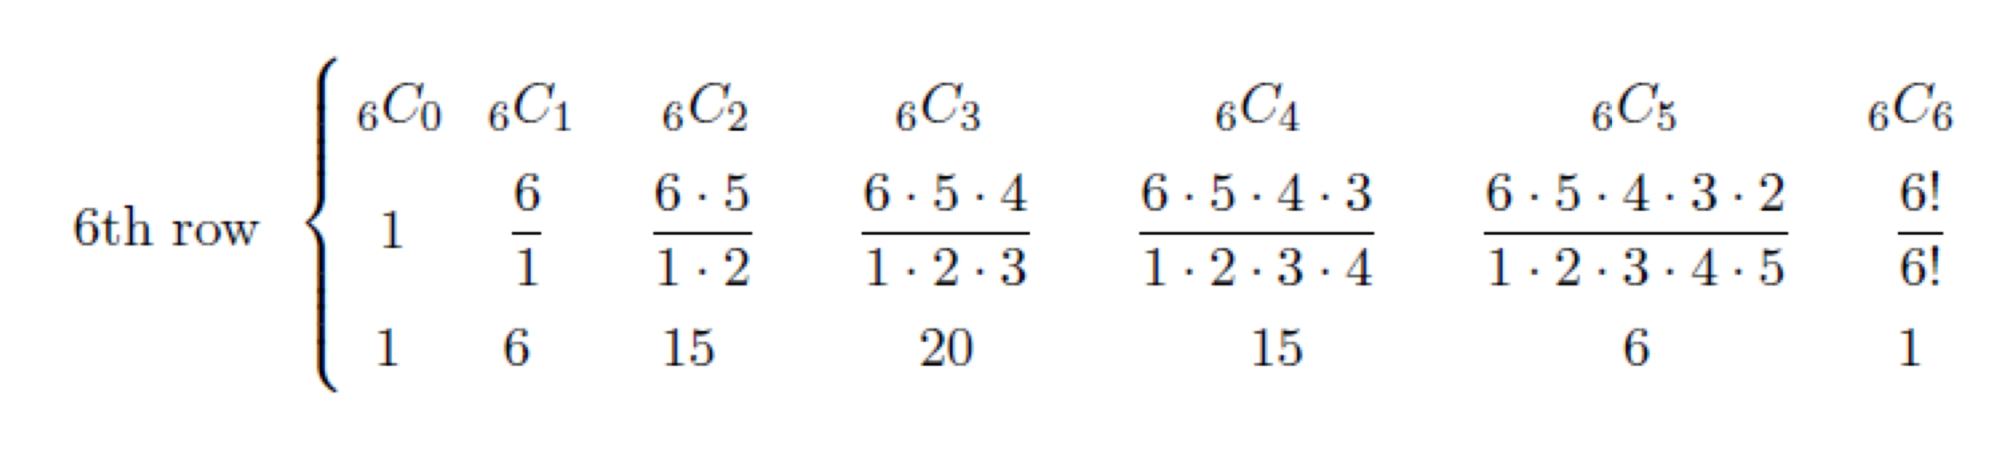
\includegraphics[width=0.6\linewidth]{./assets/binomialExpansion.png}
\end{center}

This theory is based on the Pascal's Triangle and the numbers of row $n$ correspond to the coefficients of each element of the expanded term.

We can calculate the coefficient of each part of the expanded term $k$ with combinatorics as follows: $\displaystyle {n\choose k}$

\begin{formula}[]{Binomial Expansion}
    \textbf{\textit{\underbar{In general:}}}
    \[
        (a + b)^n = 1a^nb^0 + {n\choose 1} a^{n-1}b^{1} + {n\choose 2} a^{n-2}b^{2} + \ldots + {n\choose n - 1} a^{1}b^{n - 1} + {n\choose n} a^{0}b^{n}
    \]
\end{formula}


\subsection{Overview}
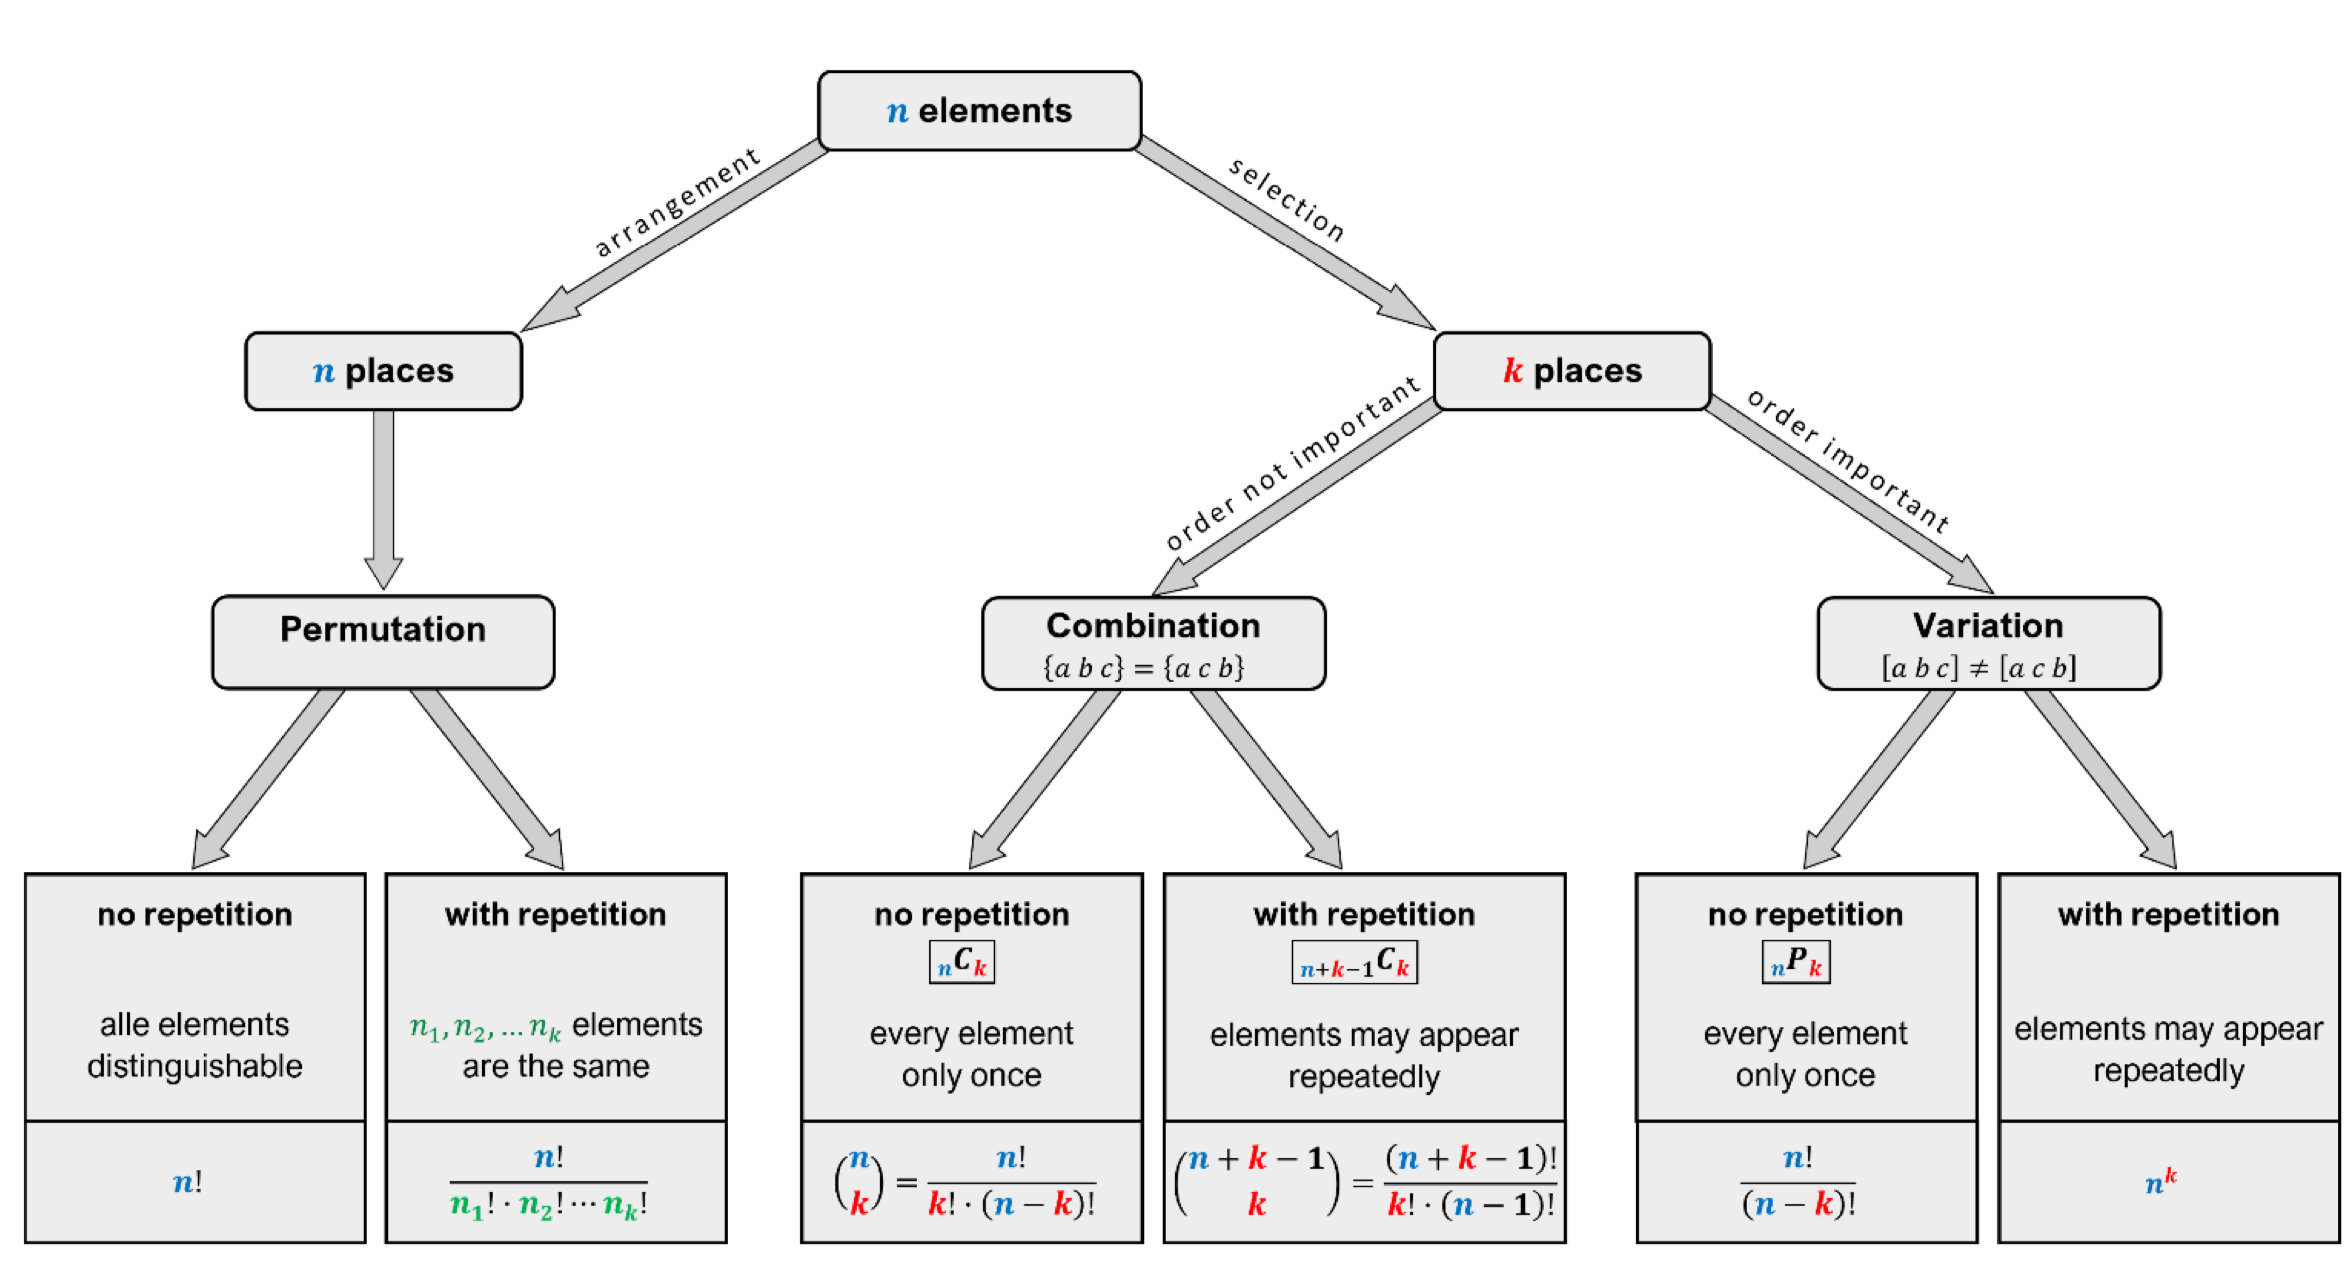
\includegraphics[width=1\linewidth]{./assets/overview.png}



% Probability
\newsection
\section{Introduction}

\subsection{Sufficiency \& Necessity}
\begin{definition}[]{Sufficiency}
    A condition $P$ is called \textit{sufficient} for $Q$ if knowing $P$ is true is enough evidence to conclude that $Q$ is true.

    This is equivalent to saying $Q \Rightarrow P$.
\end{definition}

\begin{definition}[]{Necessity}
    A condition $P$ is called \textit{necessary} for $Q$ if $Q$ cannot occur unless $P$ is true, but doesn't imply that $Q$ is true, only that it is false if $P$ is false.

    This is equivalent to saying $P \Rightarrow Q$
\end{definition}

\subsection{Asymptotic Growth}
$f$ grows asymptotically slower than $g$ if $\displaystyle\lim_{m \rightarrow \infty} \frac{f(m)}{g(m)} = 0$.
We can remark that $f$ is upper-bounded by $g$, thus $f \leq \tco{g}$ and we can say $g$ is lower bounded by $f$, thus $g \geq \tcl{f}$.
If two functions grow equally fast asymptotically, $\tct{f} = g$


\subsection{Runtime evaluation}
Identify the basic operations (usually given by the task), then count how often they are called and express that as a function in $n$.
It is easier to note that in sum notation, then simplify that sum notation into a formula not containing any summation symbols.


% ────────────────────────────────────────────────────────────────────
\subsection{Tips for Converting Summation Notation into Summation-Free Notation}

\subsubsection{Identify the Pattern:}
\begin{itemize}
    \item Examine the summand.
    \item Look for patterns related to the index variable (usually $i$, $j$, etc.). Is it a linear function, a power of $i$, a combination?
\end{itemize}


\subsubsection{Arithmetic Series Formula}
If the summand is a simple arithmetic progression (e.g., $a + bi$ where $a$ and $b$ are constants), use the formula:
\[
    \sum_{i=m}^{n} (a + bi) = (n - m + 1)\left(a + b\frac{m + n}{2}\right)
\]


\subsubsection{Power Rule for Sums}
\begin{itemize}
    \item For sums involving powers of $i$, you can use the following pattern:
          \[
              \sum_{i=1}^{n} i^k = \frac{n^{k+1}}{k+1}
          \]
    \item Remember that this rule only applies when the index starts at 1.
\end{itemize}


\subsubsection{Telescoping Series}
Look for terms in consecutive elements of the summand that cancel out, leaving a simpler expression after expanding. This is particularly helpful for fractions and ratios.


\subsubsection{Geometric Series Formula}
For sums involving constant ratios (e.g., $a \cdot r^i$ where $r$ is the common ratio), use:
\[
    \sum_{i=0}^{n} a \cdot r^i = a \frac{1 - r^{n+1}}{1-r}
\]


\subsubsection{Gaussian Formula}
If $S$ is an arithmetic series with $n$ terms, then $S = \frac{n}{2} * (a + 1)$


\subsubsection{Examples}
The only other way (other than learning these tips) in which you are going to get better at this is by parctising.
Work through examples, starting with simpler ones and moving towards more complex expressions.


\fhlc{Aquamarine}{Example:}

Let's convert the summation: $\sum_{i=1}^{5} i$

\begin{enumerate}
    \item \textbf{Pattern:} The summand is simply $i$, which represents a linear arithmetic progression.

    \item \textbf{Arithmetic Series Formula:} Applying the formula with $a = 1$, $b = 1$, $m = 1$, and $n = 5$:
          \[
              \sum_{i=1}^{5} i = (5 - 1 + 1)\left(1 + 1 \cdot \frac{1 + 5}{2}\right) = 5 \cdot 3 = 15
          \]
\end{enumerate}

Therefore, the summation evaluates to $15$.

\subsection{Specific examples}
\begin{align*}
    \frac{n}{\log(n)} \geq \Omega(\sqrt{n}) \Leftrightarrow \sqrt{n} \leq \tco{\frac{n}{\log(n)}}
\end{align*}

\newpage
\subsection{Conditional Probability}
\setcounter{all}{8}
\begin{definition}[]{Conditional Probability}
    Let $A, B$ be events, with $\Pr[B] > 0$. The \textit{conditional probability} $\Pr[A|B]$ of $A$ given $B$ is defined as
    \[
        \Pr[A|B] := \frac{\Pr[A \cap B]}{\Pr[B]}
    \]
    We may also rewrite the above as
    \[
        \Pr[A \cap B] = \Pr[B|A] \cdot \Pr[A] = \Pr[A|B] \cdot \Pr[B]
    \]
\end{definition}

\setcounter{all}{10}
\begin{theorem}[]{Multiplication law}
    Let $A_1, \ldots, A_n$ be events. If $\Pr[A_1 \cap \ldots \cap A_n] > 0$, we have
    \[
        \Pr[A_1 \cap \ldots \cap A_n] = \Pr[A_1] \cdot \Pr[A_2|A_1] \cdot \Pr[A_3|A_1 \cap A_2] \cdot \ldots \cdot \Pr[A_n|A_1 \cap \ldots \cap A_n]
    \]
\end{theorem}

The proof of the above theorem is based on the definition of conditional probability. If we rewrite $\Pr[A_1] = \frac{\Pr[A_1]}{1}$, apply the definition of $\Pr[A_2 | A_1]$, and do the same to all subsequent terms, the equation simplifies to $\Pr[A_1 \cap \ldots \cap A_n]$


\fhlc{Cyan}{Use:} The law of total probability is used, as the name implies, to calculate the total probability of all possible ways in which an even $B$ can occur.
\setcounter{all}{13}
\begin{theorem}[]{Law of total probability}
    Let $A_1, \ldots, A_n$ be relatively disjoint events and let $B \subseteq A_1 \cup \ldots \cup A_n$. We then have
    \[
        \Pr[B] = \sum_{i = 1}^{n} \Pr[B|A_i] \cdot \Pr[A_i]
    \]
    The same applies for $n = \infty$. Then, $B = \bigcup_{i = 1}^{\infty} A_i$
\end{theorem}

Using the previously defined theorem, we get Bayes' Theorem

\setcounter{all}{15}
\begin{theorem}[]{Bayes' Theorem}
    Let $A_1, \ldots, A_n$ be relatively disjoint events and let $B \subseteq A_1 \cup \ldots \cup A_n$ be an event with $\Pr[B] > 0$. Then for each $i = 1, \ldots, n$, we have
    \[
        \Pr[A_i|B] = \frac{\Pr[A_i \cap B]}{\Pr[B]} = \frac{\Pr[B|A_i] \cdot \Pr[A_i]}{\sum_{j = 1}^{n} \Pr[B|A_j] \cdot \Pr[A_j]}
    \]
    The same applies for $n = \infty$. Then $B = \bigcup_{i = 1}^{\infty} A_i$
\end{theorem}

\fhlc{Cyan}{Use:} Bayes' Theorem is commonly used to calculate probabilities on different branches or in other words, to rearrange conditional probabilities. The sum in the denominator represents all posible paths to the event summed up

\inlineex \hspace{0mm} Assume we want to find the probability that event $X$ happened given that event $Y$ happened. \textbf{Important:} Event $X$ happened \textit{before} event $Y$ happened and we do \textit{not} know the probability of $X$. Therefore we have $\Pr[X|Y]$ as the probability. But we don't actually know that probability, so we can use Bayes' Theorem to restate the problem in probabilities we can (more) easily determine.

\newpage
\subsection{Independence}
\setcounter{all}{18}
\fancydef{Independence of two events} Two events $A$ and $B$ are called \textbf{independent} if
\[
    \Pr[A \cap B] = \Pr[A] \cdot \Pr[B]
\]

\setcounter{all}{22}
\begin{definition}[]{Independence}
    Events $A_1, \ldots, A_n$ are called \textit{independent}, if for all subsets $I \subseteq \{1, \ldots, n\}$ with $I = \{i_1, \ldots, i_k\}$ and $|I| = k$, we have that
    \[
        \Pr[A_{i_1} \cap \ldots \cap A_{i_k}] = \Pr[A_{i_1}] \cdot \ldots \cdot \Pr[A_{i_k}]
    \]
\end{definition}

The same in simpler terms: If all events $A_1, \ldots, A_n$ are relatively disjoint, they are independent. We can determine if they are, if the probability of the intersection of all events is simply their individual probabilities multiplied with each other.

\begin{lemma}[]{Independence}
    Events $A_1, \ldots, A_n$ are independent if and only if for all $(s_1, \ldots, s_n) \in \{0, 1\}^n$ we have
    \[
        \Pr[A_1^{s_1} \cap \ldots \cap A_n^{s_n}] = \Pr[A_1^{s_1}] \cdot \ldots \cdot \Pr[A_n^{s_n}]
    \]
    where $A_i^{0} = \overline{A_i}$ (i.e. $s_i = 0$) and $A_i^{1} = A_i$ (i.e. $s_i = 1$)
\end{lemma}
$\{0, 1\}^n$ is the space of $n$-bit binary numbers, representing subsets of the sample space, each of them being any of the subsets intersected with up to $n$ other subsets

The $s_i$ in this expression are very straight forward to understand as simply indicating if we consider the event or its complement. 

\fancylemma{Let $A$, $B$ and $C$ be independent events. Then, $A\cap B$ and $C$ as well $A \cup B$ and $C$ are independent}

In this lecture, we are always going to assume that we can use actual random numbers, not just pseudo random numbers that are generated by PRNGs (Pseudo Random Number Generators).

\newsection
\subsection{Random Variables}
\setcounter{all}{25}
\begin{definition}[]{Random Variable}
    A \textit{random variable} is an image $\mathcal{X}: \Omega \rightarrow \R$ that maps the sample space to a real number.

    The range $W_{\mathcal{X}} := \mathcal{X}(\Omega) = \{ x \in \R : \forall \omega \in \Omega \text{ with } \mathcal{X}(\omega) = x \}$'s countability depends on the countability of $\Omega$, and is either \textit{countable} or \textit{countably infinite}
\end{definition}

\begin{scriptsize}
    \textit{For those who don't have an intuition for what a random variable actually is: See Section \ref{sec:random-var-details}.}
\end{scriptsize}

Often times when looking at random variables, we are interested in the probabilities at which $\mathcal{X}$ takes certain values.
We write either $\mathcal{X}^{-1}(x_i)$ or more intuitively $\mathcal{X} = x_i$. Analogously, we have (short: $\Pr[``\mathcal{X} \leq x_i'']$ as $\Pr[\mathcal{X} \leq x_i]$)
\[
    \Pr[``\mathcal{X} \leq x_i''] = \sum_{x \in W_{\mathcal{X}} : x \leq x_i} \Pr[``\mathcal{X} = x''] = \Pr[\{ \omega \in \Omega : \mathcal{X}(\omega) \leq x_i \}]
\]
From this notation, we easily get two real functions.
We call $f_{\mathcal{X}}: \R \rightarrow [0, 1]$ for which $x \mapsto \Pr[\mathcal{X} = x]$ the \textbf{\textit{probability mass function}} (PMF, Dichtefunktion) of $\mathcal{X}$, which maps a real number to the probability that the random variable takes this value.

The \textbf{\textit{cumulative distribution function}} (CDF, Verteilungsfunktion) of $\mathcal{X}$ is a function, which maps a real number to the probability that the value taken by the random variable is lower than, or equal to, the real number.
Often times it suffices to state the PMF of the random variable (since we can easily derive the CDF from it)
\[
    F_{\mathcal{X}} : \R \rightarrow [0, 1], \mediumhspace x\rightarrow \Pr[\mathcal{X} \leq x] = \sum_{x' \in W_{\mathcal{X}} : x' \leq x} \Pr[\mathcal{X} = x'] = \sum_{x' \in W_{\mathcal{X}} : x' \leq x} f_{\mathcal{X}}(x')
\]


\subsubsection{Expected value}
\setcounter{all}{27}
\begin{definition}[]{Expected Value}
    The \textit{expected value} $\E[\mathcal{X}]$ describes the average value the random variable $\mathcal{X}$ takes.

    We define the \textit{expected value} $\E[\mathcal{X}]$ as
    \[
        \E[\mathcal{X}] := \sum_{x \in W_{\mathcal{X}}} x \cdot \Pr[\mathcal{X} = x]
    \]
    only if the sum converges absolutely. Otherwise, the \textit{expected value} is undefined. This is trivially true for finite sample spaces.
\end{definition}
\begin{scriptsize}
    In this lecture, only random variables with an expected value are covered, so that condition does not need to be checked here
\end{scriptsize}

\setcounter{all}{29}
Alternative to the above definition over the elements of the range of the random variable, we can also define it as
\begin{lemma}[]{Expected Value}
    If $\mathcal{X}$ is a random variable, we have
    \[
        \E[\mathcal{X}] = \sum_{\omega \in \Omega} \mathcal{X}(\omega) \cdot \Pr[\omega]
    \]
\end{lemma}

If the range of the random variable consists only of non-zero integers, we can calculate the expected value with the following formula
\begin{theorem}[]{Expected Value}
    Let $\mathcal{X}$ be a random variable with $W_{\mathcal{X}} \subseteq \N_0$. We then have
    \begin{align*}
        \E[\mathcal{X}] = \sum_{i = 1}^{\infty} \Pr[\mathcal{X} \geq i]
    \end{align*}
\end{theorem}

\newpage
\fhlc{Cyan}{Conditional Random Variables}

\begin{definition}[]{Conditional Random Variable}
    Let $\mathcal{X}$ be a random variable and let $A$ be an event with $\Pr[A] > 0$
    \begin{align*}
        \Pr[(\mathcal{X} | A) \leq x] = \Pr[X \leq x | A] = \frac{\Pr[\{\omega \in A : \mathcal{X}(\omega) \leq x\}]}{\Pr[A]}
    \end{align*}
\end{definition}

\begin{theorem}[]{Expected Value (Conditional)}
    Let $\mathcal{X}$ be a random variable. For relatively disjoint events $A_1, \ldots, A_n$ with $A_1 \cup \ldots \cup A_n = \Omega$ and $\Pr[A_1], \ldots, \Pr[A_n] > 0$, we have (analogously for $n = \infty$)
    \begin{align*}
        \E[\mathcal{X}] = \sum_{i = 1}^{n} \E[\mathcal{X} | A_i] \cdot \Pr[A_i]
    \end{align*}
\end{theorem}

\fhlc{Cyan}{Linearity of the expected value}

We can calculate the expected value of a sum of any number of random variables $\mathcal{X}_1, \ldots, \mathcal{X}_n : \Omega \rightarrow \R$ simply by summing the expected values of each of the random variables $\mathcal{X}_i$

\begin{theorem}[]{Linearity of expected value}
    Given random variables $\mathcal{X}_1, \ldots, \mathcal{X}_n$ and let $\mathcal{X} := a_1 \mathcal{X}_1 + \ldots + a_n \mathcal{X}_n + b$ for any $a_1, \ldots, a_n, b \in \R$, we have
    \begin{align*}
        \E[\mathcal{X}] = a_1 \cdot \E[\mathcal{X}_1] + \ldots + a_n \cdot \E[\mathcal{X}_n] + b
    \end{align*}
\end{theorem}

Very simply with two random variables $X$ and $Y$, we have $\E[X + Y] = \E[X] + \E[Y]$

\setcounter{all}{35}
\begin{definition}[]{Indicator Variable}
    We use \textit{indicator variables} to formalize the probability that an event $A$ occurs using the expected value

    For an event $A \subseteq \Omega$ the accompanying indicator variable $\mathcal{X}_A$ is given by
    \begin{align*}
        \mathcal{X}_A(\omega) := \begin{cases}
                                     1 & \text{if } \omega \in A \\
                                     0 & \text{else }
                                 \end{cases}
    \end{align*}
    For the expected value of $\mathcal{X}_A$ we have: $\E[\mathcal{X}_A] = \Pr[A]$
\end{definition}
We can now prove the Inclusion-Exclusion-Principle using a fairly simple proof. See Example 2.36 in the script for it.

\fhlc{Cyan}{Use:} We use the indicator variable for experiments where we perform a certain action numerous times where each iteration does not (or does for that matter) depend on the previous outcome.


\newpage
\subsubsection{Variance}
Even though two random variables may have the same expected value, they can still be significantly different. The Variance describes the dispersion of the results, or how far off the expected value the different values are maximally (up to a certain limit, that is)

\setcounter{all}{39}
\begin{definition}[]{Variance}
    For a random variable $\mathcal{X}$ with $\mu = \E[\mathcal{X}]$, the \textit{variance} $\text{Var}[\mathcal{X}]$ is given by
    \begin{align*}
        \text{Var}[\mathcal{X}] := \E[(\mathcal{X} - \mu)^2] = \sum_{x \in W_{\mathcal{X}}} (x - \mu)^2 \cdot \Pr[\mathcal{X} = x]
    \end{align*}

    $\sigma := \sqrt{\text{Var}[\mathcal{X}]}$ is called the \textit{standard deviation} of $\mathcal{X}$
\end{definition}

\begin{theorem}[]{Variance (easier)}
    For any random variable $\mathcal{X}$ we have
    \[
        \text{Var}[\mathcal{X}] = \E[\mathcal{X}^2] - \E[\mathcal{X}]^2
    \]
\end{theorem}
We also have
\begin{theorem}[]{Variance}
    For any random variable $\mathcal{X}$ and $a, b \in \R$ we have
    \[
        \text{Var}[a \cdot \mathcal{X} + b] = a^2 \cdot \text{Var}[\mathcal{X}]
    \]
\end{theorem}
The moments of a random variable are given by the expected value and the variance.
\begin{definition}[]{Moment}
    The \textbf{\textit{$k$th moment}} of a random variable $\mathcal{X}$ is $\E[\mathcal{X}^k]$ whereas $\E[(\mathcal{X} - \E[\mathcal{X}])^k]$ is called the \textbf{\textit{$k$th central moment}}.
\end{definition}
\shade{gray}{Note} The expected value is thus the first moment and the variance the second central moment.


\subsubsection{Intuition}
\label{sec:random-var-details}
If you struggle to imagine what a random variable $\mathcal{X}$ is, or what for example $\mathcal{X}^2$ is, read on. 
As definition 3.25 states, a random variable is a function, which is why people tend to get confused. 
It is not a variable in the normal way of understanding. 

With that in mind, things like $\mathcal{X}^2$ makes much more sense, as it's simply the result of the function squared, which then makes theorem 3.40 make much more sense, given the definition of the expected value.

Of note is that remembering the summation formulas for the variance (or knowing how to get to it) is handy for the exam, as that formula is not listed on the cheat-sheet provided by the teaching team as of FS25. 
Deriving it is very easy though, as it's simply applying the expected value definition to the initial definition, which is listed on the cheat-sheet.

% Page 126 (actual)
\newpage
\subsection{Discrete distribution}
\subsubsection{Bernoulli-Distribution}
A random variable $\mathcal{X}$ with $W_{\mathcal{X}}$ is called \textit{\textbf{Bernoulli distributed}} if and only if its probability mass function is of form
\[
    f_{\mathcal{X}}(x) = \begin{cases}
        p     & x = 1       \\
        1 - p & x = 0       \\
        0     & \text{else}
    \end{cases}
\]
The parameter $p$ is called the probability of success (Erfolgswahrscheinlichkeit). Bernoulli distribution is used to describe boolean events (that can either occur or not). It is the trivial case of binomial distribution with $n = 1$. If a random variable $\mathcal{X}$ is Bernoulli distributed, we write
\[
    \mathcal{X} \sim \text{Bernoulli}(p)
\]
and we have
\[
    \E[\mathcal{X}] = p \hspace{1cm} \text{and} \hspace{1cm} \text{Var}[\mathcal{X}] = p(1 - p)
\]

\subsubsection{Binomial Distribution}
If we perform a Bernoulli trial repeatedly (e.g. we flip a coin $n$ times), the number of times we get one of the outcomes is our random variable $\mathcal{X}$ and it is called \textbf{\textit{binomially distributed}} and we write
\[
    \mathcal{X} \sim \text{Bin}(n, p)
\]
and we have
\[
    \E[\mathcal{X}] = np \hspace{1cm} \text{and} \hspace{1cm} \text{Var}[\mathcal{X}] = np(1 - p)
\]


\subsubsection{Geometric Distribution}
If we have an experiment that is repeated until we have achieved success, where the probability of success is $p$, the number of trials (which is described by the random variable $\mathcal{X}$) is \textbf{\textit{geometrically distributed}}. We write
\[
    \mathcal{X} \sim \text{Geo}(p)
\]
The density function is given by
\[
    f_{\mathcal{X}}(i) = \begin{cases}
        p(1 - p)^{i - 1} & \text{for } i \in \N \\
        0                & \text{else}
    \end{cases}
\]
whilst the expected value and variance are defined as
\[
    \E[\mathcal{X}] = \frac{1}{p} \hspace{1cm} \text{and} \hspace{1cm} \text{Var}[\mathcal{X}] = \frac{1 - p}{p^2}
\]
The cumulative distribution function is given by
\[
    F_{\mathcal{X}}(n) = \Pr[\mathcal{X} \leq n] = \sum_{i = 1}^{n} \Pr[\mathcal{X} = i] = \sum_{i = 1}^{n} p(1 - p)^{i - 1} = 1 - (1 - p)^n
\]
\shade{gray}{Note} Every trial in the geometric distribution is unaffected by the previous trials
\setcounter{all}{45}
\begin{theorem}[]{Geometric Distribution}
    If $\mathcal{X} \sim \text{Geo}(p)$, for all $s, t \in \N$ we have
    \[
        \Pr[\mathcal{X} \geq s + t | X > s] = \Pr[X \geq t]
    \]
\end{theorem}

\newpage
\fhlc{cyan}{Coupon Collector problem}

First some theory regarding waiting for the $n$th success. The probability mass function is given by $f_{\mathcal{X}}(x) = \begin{pmatrix}z - 1\\ n - 1\end{pmatrix} \cdot p^n \cdot (1- p)^{z - n}$ whereas the expected value is given by $\displaystyle\E[\mathcal{X}] = \sum_{i = 1}^{n} \E[\mathcal{X}_i] = \frac{n}{p}$

The coupon collector problem is a well known problem where we want to collect all coupons on offer. How many coupons do we need to obtain on average to get one of each? We will assume that the probability of getting coupon $i$ is equal to all other coupons and getting a coupon doesn't depend on what coupons we already have (independence)

Let $\mathcal{X}$ be a random variable representing the number of purchases to the completion of the collection. We split up the time into separate phases, where $\mathcal{X}$ is the number of coupons needed to end phase $i$, which ends when we have found one of the $n - i + 1$ coupons not previously collected (i.e. we got a coupon we haven't gotten yet)

Logically, $\mathcal{X} = \sum_{i = 1}^{n} \mathcal{X}_i$. We can already tell from the experiment we are conducting that it is going to be geometrically distributed and thus the probability of success is going to be $p = \frac{n - i + 1}{n}$ and we have $\E[\mathcal{X}_i] = \frac{n}{n - i + 1}$

With that, let's determine
\[
    \E[\mathcal{X}] = \sum_{i = 1}^{n} \E[\mathcal{X}_i] = \sum_{i = 1}^{n} \frac{n}{n - i + 1} = n \cdot \sum_{i = 1}^{n} \frac{1}{i} = n \cdot H_n
\]
where $H_n := \sum_{i = 1}^{n} \frac{1}{i}$ is the $n$th harmonic number, which we know (from Analysis) is $H_n = \ln(n) +$\tco{1}, thus we have $\E[\mathcal{X}] = n \cdot \ln(n) +$\tco{n}.

The idea of the transformation is to reverse the $(n - i + 1)$, so counting up instead of down, massively simplifying the sum and then extracting the $n$ and using the result of $H_n$ to fully simplify


\subsubsection{Poisson distribution}
The \textbf{\textit{Poisson distribution}} is applied when there is only a small likelihood that an event occurs, but since the cardinality of the sample space in question is large, we can expect at least a few events to occur.
We write
\[
    \mathcal{X} \sim \text{Po}(\lambda)
\]
An example for this would be for a person to be involved in an accident over the next hour. The probability mass function is given by
\[
    f_{\mathcal{X}}(i) = \begin{cases}
        \frac{e^{-\lambda}\lambda^i}{i!} & \text{for } i \in \N_o \\
        0                                & \text{else}
    \end{cases}
    \hspace{1cm} \text{and} \hspace{1cm} \E[\mathcal{X}] = \text{Var}[\mathcal{X}] = \lambda
\]

\shade{cyan}{Using the Poisson distribution as limit for the binomial distribution}

We can approximate the binomial distribution using the Poisson distribution if we have large $n$ and small constant $np$. $\lambda = \E[\mathcal{X}] = np$ in that case.

\newpage
\subsection{Multiple random variables}
There are times when we are interested in the outcomes of multiple random variables simultaneously. For two random variables $\mathcal{X}$ and $\mathcal{Y}$, we evaluate probabilities of type
\[
    \Pr[\mathcal{X} = x, \mathcal{Y} = y] = \Pr[\{ \omega \in \Omega : \mathcal{X}(\omega) = x, \mathcal{Y}(\omega) = y \}]
\]
Here $\Pr[\mathcal{X} = x, \mathcal{Y} = y]$ is a shorthand notation for $\Pr[``\mathcal{X} = x'' \cap ``\mathcal{Y} = y'']$

We define the \textit{common probability mass function} $f_{\mathcal{X}, \mathcal{Y}}$ by
\[
    f_{\mathcal{X}, \mathcal{Y}}(x, y) := \Pr[\mathcal{X} = x, \mathcal{Y} = y]
\]
We can also get back to the individual probability mass of each random variable
\begin{align*}
    f_{\mathcal{X}} = \sum_{y \in W_{\mathcal{Y}}} f_{\mathcal{X}, \mathcal{Y}}(x, y) \hspace{1cm} \text{or} \hspace{1cm} f_{\mathcal{Y}}(y) = \sum_{x \in W_{\mathcal{X}}} f_{\mathcal{X}, \mathcal{Y}}(x, y)
\end{align*}
We hereby call $f_{\mathcal{X}}$ and $f_{\mathcal{Y}}$ \textit{marginal density} (Randdichte)

We define the \textbf{\textit{common cumulative distribution function}} by
\begin{align*}
    F_{\mathcal{X}, \mathcal{Y}}(x, y) := \Pr[\mathcal{X} \leq x, \mathcal{Y} \leq y] = \Pr[\{ \omega \in \Omega : \mathcal{X}(\omega) \leq x, \mathcal{Y} \leq y \}] = \sum_{x' \leq x} \sum_{y' \leq y} f_{\mathcal{X}, \mathcal{Y}}(x', y')
\end{align*}

Again, we can use marginal density
\begin{align*}
    F_{\mathcal{X}}(x) = \sum_{x'\leq x} f_{\mathcal{X}}(x') = \sum_{x' \leq x} \sum_{y \in W_{\mathcal{Y}}} f_{\mathcal{X}, \mathcal{Y}}(x', y)
    \hspace{5mm} \text{and} \hspace{5mm}
    F_{\mathcal{Y}}(y) = \sum_{y'\leq y} f_{\mathcal{Y}}(y') = \sum_{y' \leq y} \sum_{x \in W_{\mathcal{X}}} f_{\mathcal{X}, \mathcal{Y}}(x, y')
\end{align*}

\subsubsection{Independence of random variables}
\setcounter{all}{52}
\begin{definition}[]{Independence}
    Random variables $\mathcal{X}_1, \ldots, \mathcal{X}_n$ are called \textbf{\textit{independent}}
    if and only if for all $(x_1, \ldots, x_n) \in W_{\mathcal{X}_1} \times \ldots \times W_{\mathcal{X}_n}$ we have
    \begin{align*}
        \Pr[\mathcal{X}_1 = x_1, \ldots, \mathcal{X}_n = x_n] = \Pr[\mathcal{X}_1 = x_1] \cdot \ldots \cdot \Pr[\mathcal{X}_n = x_n]
    \end{align*}
    Or alternatively, using probability mass functions
    \begin{align*}
        f_{\mathcal{X}_1, \ldots \mathcal{X}_n}(x_1, \ldots, x_n) = f_{\mathcal{X}_1}(x_1) \cdot \ldots \cdot f_{\mathcal{X}_n}(x_n)
    \end{align*}
    In words, this means that for independent random variables, their common density is equal to the product of the individual marginal densities
\end{definition}
The following lemma shows that the above doesn't only hold for specific values, but also for sets
\begin{lemma}[]{Independence}
    Let $\mathcal{X}_1, \ldots, \mathcal{X}_n$ be independent random variables and let $S_1, \ldots, S_n \subseteq \R$ be any set, then we have
    \begin{align*}
        \Pr[\mathcal{X}_1 \in S_1, \ldots, \mathcal{X}_n \in S_n] = \Pr[\mathcal{X}_1 \in S_1] \cdot \ldots \cdot \Pr[\mathcal{X}_n \in S_n]
    \end{align*}
\end{lemma}

\begin{corollary}[]{Independence}
    Let $\mathcal{X}_1, \ldots, \mathcal{X}_n$ be independent random variables and let $I = \{i_1, \ldots, i_k\} \subseteq [n]$, then $\mathcal{X}_{i_1}, \ldots, \mathcal{X}_{i_k}$ are also independent
\end{corollary}

\begin{theorem}[]{Independence}
    Let $f_1, \ldots, f_n$ be real-valued functions ($f_i : \R \rightarrow \R$ for $i = 1, \ldots, n$). If the random variables $X_1, \ldots, X_n$ are independent, then this also applies to $f_1(\mathcal{X}_1), \ldots, f_n(\mathcal{X}_n)$
\end{theorem}


\subsubsection{Composite random variables}
Using functions we can combine multiple random variables in a sample space.

\setcounter{all}{58}
\begin{theorem}[]{Two random variables}
    For two independent random variables $\mathcal{X}$ and $\mathcal{Y}$, let $\mathcal{Z} := \mathcal{X} + \mathcal{Y}$. Then we have
    \begin{align*}
        f_{\mathcal{Z}}(z) = \sum_{x \in W_{\mathcal{X}}} f_{\mathcal{X}} \cdot f_{\mathcal{Y}}(z - x)
    \end{align*}
\end{theorem}
We call, analogously to the terms used for power series, $f_{\mathcal{Z}}(z)$ ``convolution''


\subsubsection{Moments of composite random variables}
\setcounter{all}{60}
\begin{theorem}[]{Linearity of the expected value}
    For random variables $\mathcal{X}_1, \ldots, \mathcal{X}_n$ and $\mathcal{X} := a_1 \mathcal{X}_1 + \ldots + a_n \mathcal{X}_n$ with $a_1, \ldots, a_n \in \R$ we have
    \begin{align*}
        \E[\mathcal{X}] = a_1 \E[\mathcal{X}_1] + \ldots + a_n \E[\mathcal{X}_n]
    \end{align*}
\end{theorem}
There are no requirements in terms of independence of the random variables, unlike for the multiplicativity

\begin{theorem}[]{Multiplicativity of the expected value}
    For independent random variables $\mathcal{X}_1, \ldots, \mathcal{X}_n$ we have
    \begin{align*}
        \E[\mathcal{X}_1 \cdot \ldots \cdot \mathcal{X}_n] = \E[\mathcal{X}_1] \cdot \ldots \cdot \E[\mathcal{X}_n]
    \end{align*}
\end{theorem}

\begin{theorem}[]{Variance of multiple random variables}
    For independent random variables $\mathcal{X}_1, \ldots, \mathcal{X}_n$ and $\mathcal{X} = \mathcal{X}_1 + \ldots + \mathcal{X}_n$ we have
    \begin{align*}
        \text{Var}[\mathcal{X}] = \text{Var}[\mathcal{X}_1] + \ldots + \text{Var}[\mathcal{X}_n]
    \end{align*}
\end{theorem}


\subsubsection{Wald's Identity}
Wald's identity is used for cases where the number of summands is not a constant, commonly for algorithms that repeatedly call subroutines until a certain result is attained.
The time complexity of such an algorithm can be approximated by splitting up the algorithm into phases, where each phase is a call of the subroutine.
The number of calls to the subroutine, thus the number of phases, is usually not deterministic in that case but rather bound to a random variable.

\setcounter{all}{65}
\begin{theorem}[]{Wald's Identity}
    Let $\mathcal{N}$ and $\mathcal{X}$ be two independent random variables with $W_{\mathcal{N}} \subseteq \N$. Let
    \begin{align*}
        \mathcal{Z} := \sum_{i = 1}^{\mathcal{N}}\mathcal{X}_i
    \end{align*}
    where $\mathcal{X}_1, \mathcal{X}_2, \ldots$ are independent copies of $\mathcal{X}$. Then we have
    \begin{align*}
        \E[\mathcal{Z}] = \E[\mathcal{N}] \cdot \E[\mathcal{X}]
    \end{align*}
\end{theorem}

\newpage
\subsection{Approximating probabilities}
Since it can be very expensive to calculate the true probabilities in some cases, we will now cover some tools that allow us to approximate the probabilities using upper or lower bounds.

\subsubsection{Markov's \& Chebyshev's inequalities}
\setcounter{all}{67}
\begin{theorem}[]{Markov's inequality}
    Let $\mathcal{X}$ be a random variable that may only take non-negative values. Then for all $t > 0 \in \R$, we have
    \begin{align*}
        \Pr[\mathcal{X} \geq t] \leq \frac{\E[\mathcal{X}]}{t} \Longleftrightarrow \Pr[\mathcal{X} \geq t \cdot \E[\mathcal{X}]] \leq \frac{1}{t}
    \end{align*}
\end{theorem}
Markov's inequality is fairly straight forward to prove, and it already allows us to make some useful statements, like that for the coupon collector problem, we only need to make more than $100 n \log(n)$ purchases with probability $\frac{1}{100}$. The following inequality usually gives a much more precise bound than Markov's inequality

\begin{theorem}[]{Chebyshev's inequality}
    Let $\mathcal{X}$ be a random variable and $t > 0 \in\R$. Then we have
    \begin{align*}
        \Pr[|\mathcal{X} - \E[\mathcal{X}| \geq t]] \leq \frac{\text{Var}[\mathcal{X}]}{t^2} \Longleftrightarrow \Pr[|\mathcal{X} - \E[\mathcal{X}]| \geq t \cdot \sqrt{\text{Var}[\mathcal{X}]}] \leq \frac{1}{t^2}
    \end{align*}
\end{theorem}

A common tactic when using these is to restate the original probability $\Pr[X \geq t]$ as $\Pr[|X - \E[X]| \geq t - \E[X]]$ and then set $t = t'$ for $t' = t - \E[X]$

\subsubsection{Chernoff bounds}
The Chernoff bounds are specifically designed for Bernoulli-variables
\setcounter{all}{70}
\begin{theorem}[]{Chernoff bounds}
    Let $\mathcal{X}_1, \ldots, \mathcal{X}_n$ be independent Bernoulli-distributed random variables with $\Pr[\mathcal{X}_i = 1] = p_i$ and $\Pr[\mathcal{X}_i = 0] = 1 - p_i$. Then we have for $\mathcal{X} := \sum_{i = 1}^{n} \mathcal{X}_i$
    \begin{enumerate}[label=(\roman*)]
        \item $\Pr[\mathcal{X} \geq (1 + \delta)\E[\mathcal{X}]] \leq e^{-\frac{1}{3}\delta^2\E[\mathcal{X}]}$ \largehspace for all $0 < \delta \leq 1$
        \item $\Pr[\mathcal{X} \leq (1 - \delta)\E[\mathcal{X}]] \leq e^{-\frac{1}{2}\delta^2\E[\mathcal{X}]}$ \largehspace for all $0 < \delta \leq 1$
        \item $\Pr[\mathcal{X} \geq t] \leq 2^{-t}$ \largehspace for $t \geq 2e\E[\mathcal{X}]$
    \end{enumerate}
\end{theorem}
We determine the $\delta$ in the inequality by finding it such that $t = (1 + \delta)\E[X]$ or, for the second one, $t = (1 - \delta)\E[X]$. For the third one, no $\delta$ is required

\newpage
\fhlc{Cyan}{Algorithms}

Most algorithms for the max-flow problem use a residual network, where $\mathcal{A}_f$ is the edge-set in the residual network.

\begin{algorithm}
    \caption{\textsc{Ford-Fulkerson}}
    \begin{algorithmic}[1]
        \Procedure{Ford-Fulkerson}{$\mathcal{V}, \mathcal{A}, c, s, t$}
            \State $f \gets 0$ \Comment{Flow is constantly $0$}
            \While{$\exists s$-$t$-path $P$ in $(\mathcal{V}, \mathcal{A}_f)$} \Comment{Augmenting path}
                \State Increase flow along $P$ by minimum residual capacity in $P$
            \EndWhile
            \State \Return $f$ \Comment{Maximum flow}
        \EndProcedure
    \end{algorithmic}
\end{algorithm}

The problem with this algorithm is that it may not terminate for irrational capacities. If we however only consider integral networks without bidirectional edges, it can be easily seen that if we denote $U \in \N$ the upper bound for capacities, the time complexity of this algorithm is \tco{nUm} where \tco{m} is the time complexity for constructing residual network.
\begin{theorem}[]{Max-Flow Algorithm}
    If in a network without bidirectional edges and all capacities integral and no larger than $U$, there is an integral max-flow we can compute in \tco{mnU}, whereas $m$ is the number of edges and $n$ the number of vertices in the network.
\end{theorem}

There are more advanced algorithms than this one that can calculate solutions to this problem faster or also for irrational numbers.
For the following two proposition, $m = |E|$ and $n = |V|$, i.e. $m$ is the number of edges and $n$ the number of vertices

\begin{proposition}[]{Capacity-Scaling}
    If in a network all capacities are integral and at most $U$, there exists an integral max-flow that can be computed in \tco{mn(1 + \log(U))}
\end{proposition}

\begin{proposition}[]{Dynamic-Trees}
    The max-flow of a flow in a network can be calculated in \tco{mn\log(n)}
\end{proposition}





% Algorithms
\newsection
\section{Algorithms}
\subsection{Graph algorithms}

\subsubsection{Long path problem}
Given a tuple $(G, B)$ where $G$ is a graph and $B \in \N_0$, we need to determine whether there exists a path of length $B$ in $G$.

This problem is another one of the infamous $\mathcal{N}\mathcal{P}$-Complete problems, for which there \textit{supposedly} doesn't exist an algorithm that can solve the problem in polynomial time.
We can show that this problem belongs to said group if we can show that we can \textit{efficiently} construct a graph $G'$ with $n' \leq 2n - 2$ vertices such that $G$ has a Hamiltonian Cycle if and only if $G'$ has a path of length $n$.

We construct a graph $G'$ from graph $G$ by selecting a vertex $v$ and replacing each edge incident to that vertex with edges that lead to newly added vertices $\hat{w_1}, \hat{w_2}, \ldots$.
$G'$ has $(n - 1) + \deg(v) \leq 2n - 2$ vertices. All the vertices $\hat{w_1}, \ldots, \hat{w_{\deg(v)}}$ all have degree $1$.

The graph $G'$ fulfills the above implication because
\begin{enumerate}[label=(\roman*)]
    \item Let $\langle v_1, v_2, \ldots, v_n, v_1 \rangle$ be a Hamiltonian cycle.
          Assume for contradiction that the resulting graph, constructed according to the description above does not contain a path of length $n$.
          Let's assume $v_1 = v$ (the vertex removed during construction). However, $\langle \hat{v_2}, v_2, \ldots, \hat{v_n}, v_n \rangle$ is a path of length $n$
    \item Let $\langle u_0, u_1, \ldots, u_n \rangle$ be a path of length $n$ in $G'$ and let $\deg(u_i) \geq 2 \smallhspace \forall i \in \{1, \ldots, n - 1\}$ These vertices hence have to be the $n - 1$ remaining vertices of $G$, thus we have $u_0 = \hat{w_i}$ and $u_n = \hat{w_j}$ two different ones of new vertices of degree $1$ in $G'$. Thus, we have $u_1 = w_i$ and $u_{n - 1} = w_j$ and we have $\langle v, u_1, \ldots, u_{n - 1}, v \rangle$, which is a Hamiltonian cycle in $G$
\end{enumerate}
Due to the construction of the graph $G'$ we can generate it from $G$ in $\tco{n^2}$ steps. We thus have:

\begin{theorem}[]{Long Path Problem}
    If we can find a \textit{long-path} in a graph with $n$ vertices in time $t(n)$, we can decide if a graph with $n$ vertices has a Hamiltonian cycle in $t(2n - 2) + \tco{n^2}$
\end{theorem}


\fhlc{Cyan}{Short long paths}

In biological applications, the long paths searched are usually small compared to $n$. It is possible to solve this problem in polynomial time if for the tuple $(G, B)$ $B = \log(n)$.

Notation and useful properties:
\begin{itemize}
    \item $[n] := \{1, 2, \ldots, n\}$. $[n]^k$ is the set of sequences over $[n]$ of length $k$ and we have $\left| [n]^k \right| = n^k$. ${[n] \choose k}$ is the set of subsets of $[n]$ of cardinality $k$ and we have $\left| {[n] \choose k} \right| = {n \choose k}$
    \item For every graph $G = (V, E)$ we have $\sum_{v \in V} \deg(v) = 2|E|$
    \item $k$ vertices (no matter if part of a path or not) can be coloured using $[k]$ in exactly $k^k$ ways whereas $k!$ of said colourings use each colour exactly once.
    \item For $c, n \in \R^+$ we have $c^{\log(n)} = n^{\log(c)}$
    \item For $n \in \N_0$ we have $\sum_{i = 0}^{n} {n \choose i} = 2^n$. (Application of binomial expansion, see \ref{sec:binomial-expansion})
    \item For $n \in \N_0$ we have $\frac{n!}{n^n} \geq e^{-n}$
    \item If we repeat an experiment with probability of success $p$ until success, $\E[\mathcal{X}] = \frac{1}{p}$ where $\mathcal{X} :=$ number of trials
\end{itemize}


\newpage
\shade{ForestGreen}{Colourful paths}

A path is called \textit{colourful} if all vertices on it are coloured differently.
For $v \in V$ and $i \in \N_0$ let's define
\begin{align*}
    P_i(v) := \left\{ S \in {[k] \choose i + 1} \smallhspace \Bigg| \smallhspace \exists \text{ path ending in $v$ coloured with $S$ colours } \right\}
\end{align*}
Thus, $P_i(v)$ contains a set $S$ of $i + 1$ colours if and only if there exists a path with vertex $v$ whose colours are the colours in $S$.
It is important to note that such a path has to be always \textit{exactly} of length $i$.

If we solve this problem for every $v \in V$, we solved our problem and we have
\begin{align*}
    \exists \text{ colourful path of length $k - 1$ } \Longleftrightarrow \bigcup_{v \in V} P_{k - 1}(v) \neq \emptyset
\end{align*}
For the algorithm, we need to also define $N(v)$ which returns the neighbours of $v$ and $\gamma: V \rightarrow [k]$ which assigns a colour to each vertex.

\begin{algorithm}
    \caption{Colourful path algorithm}
    \begin{algorithmic}[1]
        \Procedure{Colourful}{$G, i$}
            \For{\textbf{all} $v \in V$}
                \State $P_i(v) \gets \emptyset$
                \For{\textbf{all} $x \in N(v)$}
                    \For{\textbf{all} $R \in P_{i - 1}(x)$ with $\gamma(v) \notin R$}
                        \State $P_i(v) \gets P_i(v) \cup \{R \cup \{\gamma(v)\}\}$
                    \EndFor
                \EndFor
            \EndFor
        \EndProcedure
    \end{algorithmic}
\end{algorithm}
The time complexity of this algorithm is $\tco{2^k km}$. If we now have $k = \tco{\log(n)}$, the algorithm is polynomial.


\shade{ForestGreen}{Random colouring}

The idea to solve the short long path problem in polynomial time is to randomly colour the vertices using colours $[k]$, whereby $k := B + 1$ and check if there is a colourful path of length $k - 1$.
Since we are guaranteed to have a colourful path if we find one, we can develop a Las Vegas Algorithm that solves this problem. But first
\begin{theorem}[]{Random Colouring}
    Let $G$ be a graph with a path of length $k - 1$
    \begin{enumerate}[label=(\arabic*)]
        \item We have $p_{\text{success}} = \Pr[\exists \text{ colourful path of length } k - 1] \geq \Pr[P \text{ is colourful}] = \frac{k!}{k^k} \geq e^{-k}$
        \item The expected number of trials required to get a colourful path of length $k - 1$ is $\frac{1}{p_{\text{success}}} \leq e^k$
    \end{enumerate}
\end{theorem}
For our algorithm we choose a $\lambda > 1 \in \R$ and we repeat the test at most $\ceil{\lambda e^k}$. If we succeed once, we abort and output ``\textsc{Yes}''. If we haven't succeeded in any of the trials, we output ``\textsc{No}''

\begin{theorem}[]{Random Colouring Algorithm}
    \begin{itemize}
        \item Time complexity: $\tco{\lambda(2e)^k km}$
        \item If we return ``\textsc{Yes}'', the graph is \textit{guaranteed} to contain a path of length $k - 1$
        \item If we return ``\textsc{No}'', the probability of false negative is $e^{-\lambda}$
    \end{itemize}
\end{theorem}

\newsection
\section{Introduction}

\subsection{Sufficiency \& Necessity}
\begin{definition}[]{Sufficiency}
    A condition $P$ is called \textit{sufficient} for $Q$ if knowing $P$ is true is enough evidence to conclude that $Q$ is true.

    This is equivalent to saying $Q \Rightarrow P$.
\end{definition}

\begin{definition}[]{Necessity}
    A condition $P$ is called \textit{necessary} for $Q$ if $Q$ cannot occur unless $P$ is true, but doesn't imply that $Q$ is true, only that it is false if $P$ is false.

    This is equivalent to saying $P \Rightarrow Q$
\end{definition}

\subsection{Asymptotic Growth}
$f$ grows asymptotically slower than $g$ if $\displaystyle\lim_{m \rightarrow \infty} \frac{f(m)}{g(m)} = 0$.
We can remark that $f$ is upper-bounded by $g$, thus $f \leq \tco{g}$ and we can say $g$ is lower bounded by $f$, thus $g \geq \tcl{f}$.
If two functions grow equally fast asymptotically, $\tct{f} = g$


\subsection{Runtime evaluation}
Identify the basic operations (usually given by the task), then count how often they are called and express that as a function in $n$.
It is easier to note that in sum notation, then simplify that sum notation into a formula not containing any summation symbols.


% ────────────────────────────────────────────────────────────────────
\subsection{Tips for Converting Summation Notation into Summation-Free Notation}

\subsubsection{Identify the Pattern:}
\begin{itemize}
    \item Examine the summand.
    \item Look for patterns related to the index variable (usually $i$, $j$, etc.). Is it a linear function, a power of $i$, a combination?
\end{itemize}


\subsubsection{Arithmetic Series Formula}
If the summand is a simple arithmetic progression (e.g., $a + bi$ where $a$ and $b$ are constants), use the formula:
\[
    \sum_{i=m}^{n} (a + bi) = (n - m + 1)\left(a + b\frac{m + n}{2}\right)
\]


\subsubsection{Power Rule for Sums}
\begin{itemize}
    \item For sums involving powers of $i$, you can use the following pattern:
          \[
              \sum_{i=1}^{n} i^k = \frac{n^{k+1}}{k+1}
          \]
    \item Remember that this rule only applies when the index starts at 1.
\end{itemize}


\subsubsection{Telescoping Series}
Look for terms in consecutive elements of the summand that cancel out, leaving a simpler expression after expanding. This is particularly helpful for fractions and ratios.


\subsubsection{Geometric Series Formula}
For sums involving constant ratios (e.g., $a \cdot r^i$ where $r$ is the common ratio), use:
\[
    \sum_{i=0}^{n} a \cdot r^i = a \frac{1 - r^{n+1}}{1-r}
\]


\subsubsection{Gaussian Formula}
If $S$ is an arithmetic series with $n$ terms, then $S = \frac{n}{2} * (a + 1)$


\subsubsection{Examples}
The only other way (other than learning these tips) in which you are going to get better at this is by parctising.
Work through examples, starting with simpler ones and moving towards more complex expressions.


\fhlc{Aquamarine}{Example:}

Let's convert the summation: $\sum_{i=1}^{5} i$

\begin{enumerate}
    \item \textbf{Pattern:} The summand is simply $i$, which represents a linear arithmetic progression.

    \item \textbf{Arithmetic Series Formula:} Applying the formula with $a = 1$, $b = 1$, $m = 1$, and $n = 5$:
          \[
              \sum_{i=1}^{5} i = (5 - 1 + 1)\left(1 + 1 \cdot \frac{1 + 5}{2}\right) = 5 \cdot 3 = 15
          \]
\end{enumerate}

Therefore, the summation evaluates to $15$.

\subsection{Specific examples}
\begin{align*}
    \frac{n}{\log(n)} \geq \Omega(\sqrt{n}) \Leftrightarrow \sqrt{n} \leq \tco{\frac{n}{\log(n)}}
\end{align*}

\begin{definition}[]{$s$-$t$-cut}
    An $s$-$t$-cut of a network $N = (\mathcal{V}, \mathcal{A}, c, s, t)$ is a partition $P = (\mathcal{S}, \mathcal{T})$ of $\mathcal{V}$ (i.e. $\mathcal{S} \cup \mathcal{T} = \mathcal{V}$ and $\mathcal{S} \cap \mathcal{T} = \emptyset$) where $s \in \mathcal{S}$ and $t \in \mathcal{T}$.
    The capacity of a $s$-$t$-cut is then given by
    \begin{align*}
        \text{cap}(\mathcal{S}, \mathcal{T}) = \sum_{(u, w) \in (\mathcal{S} \times \mathcal{T}) \cap \mathcal{A}} c(u, w)
    \end{align*}
\end{definition}

\begin{lemma}[]{$s$-$t$-cut}
    Given $f$ is a flow and $(\mathcal{S}, \mathcal{T})$ a $s$-$t$-cut in $N = (\mathcal{V}, \mathcal{A}, c, s, t)$, we have
    \begin{align*}
        \text{val}(f) \leq \text{cap}(\mathcal{S}, \mathcal{T})
    \end{align*}
\end{lemma}


\begin{theorem}[]{Max-flow - min-cut}
    Every network $N = (\mathcal{V}, \mathcal{A}, c, s, t)$ fulfills ($f$ a flow, $(\mathcal{S}, \mathcal{T})$ an $s$-$t$-cut)
    \begin{align*}
        \max_{f \in N} \text{val}(f) = \min_{(\mathcal{S}, \mathcal{T}) \in N} \text{cap}(S, T)
    \end{align*}
\end{theorem}

It is easier to calculate the min-cut, since there are only a finite number of $s$-$t$-cuts (albeit exponentially many, i.e. $2^{|\mathcal{V}| - 2}$), thus the importance of the above theorem.
It forms the basis of the algorithms that calculate a solution to the max-flow problem.

An approach to solve the max-flow problem is to use augmenting paths, but the issue with that is that it isn't guaranteed that we will find a max flow in a finite number of steps.

\fhlc{Cyan}{Residual capacity network}

Using a residual capacity graph also known as a residual network, we can solve the max-flow problem in polynomial time.
The concept is simple, yet ingenious: It is simply a network of the remaining capacity (or the exceeded capacity) of an edge $e \in \mathcal{A}$ for a flow $f$

\begin{definition}[]{Residual Network}
    Let $N = (\mathcal{V}, \mathcal{A}, c, s, t)$ be a network without bidirectional edges and let $f$ be a flow in said network $N$. The residual network $N_f = (\mathcal{V}, \mathcal{A}_f, r_f, s, t)$ is given by
    \begin{enumerate}[label=(\arabic*)]
        \item If $e \in \mathcal{A}$ with $f(e) < c(e)$, then edge $e$ is also $\in \mathcal{A}_f$ whereas $r_f(e) := c(e) - f(e)$
        \item If $e \in \mathcal{A}$ with $f(e) > 0$ then edge $e^{\text{opp}}$ in $\mathcal{A}_f$ whereas $r_f(e^{\text{opp}}) = f(e)$
        \item Only edges as described in (1) and (2) can be found in $\mathcal{A}_f$
    \end{enumerate}

    We call $r_f(e), e \in \mathcal{A}$ the \textit{residual capacity} of edge $e$
\end{definition}

When reconstructing a network from the residual network, the original network is given by:
\begin{itemize}
    \item The capacity of an edge $(u, v)$ in the original network is the value of $(u, v)$ and $(v, u)$ in the residual network added (if applicable), where $(u, v)$ is directed \textit{towards} the target.
    \item The flow of an edge is a bit more complicated: An edge that might appear to intuitively not be part of the flow may be and vice-versa.
          Flow preservation is the key: The same amount of fluid has to enter each vertex (that is not $s$ or $t$) has to also exit it again.
          To check if an edge is part of the flow, simply see if the start vertex of the edge has an excess of fluid.
    \item If just one edge is present, the edge is flipped, if two are present, figure out which edge was part of the flow and which one is the remaining capacity.
\end{itemize}
Note: A vertex in the residual network directed towards the \textit{target} is usually the remaining capacity!

\begin{theorem}[]{Maximum Flow}
    A flow $f$ in a network $N = (\mathcal{V}, \mathcal{A}, c, s, t)$ is a maximum flow if and only if there does not exist a directed path between the source and target of the residual network.

    For every such maximum flow there exists a $s$-$t$-cut with $\text{val}(f) = \text{cap}(S, T)$
\end{theorem}

\newpage
\fhlc{Cyan}{Algorithms}

Most algorithms for the max-flow problem use a residual network, where $\mathcal{A}_f$ is the edge-set in the residual network.

\begin{algorithm}
    \caption{\textsc{Ford-Fulkerson}}
    \begin{algorithmic}[1]
        \Procedure{Ford-Fulkerson}{$\mathcal{V}, \mathcal{A}, c, s, t$}
            \State $f \gets 0$ \Comment{Flow is constantly $0$}
            \While{$\exists s$-$t$-path $P$ in $(\mathcal{V}, \mathcal{A}_f)$} \Comment{Augmenting path}
                \State Increase flow along $P$ by minimum residual capacity in $P$
            \EndWhile
            \State \Return $f$ \Comment{Maximum flow}
        \EndProcedure
    \end{algorithmic}
\end{algorithm}

The problem with this algorithm is that it may not terminate for irrational capacities. If we however only consider integral networks without bidirectional edges, it can be easily seen that if we denote $U \in \N$ the upper bound for capacities, the time complexity of this algorithm is \tco{nUm} where \tco{m} is the time complexity for constructing residual network.
\begin{theorem}[]{Max-Flow Algorithm}
    If in a network without bidirectional edges and all capacities integral and no larger than $U$, there is an integral max-flow we can compute in \tco{mnU}, whereas $m$ is the number of edges and $n$ the number of vertices in the network.
\end{theorem}

There are more advanced algorithms than this one that can calculate solutions to this problem faster or also for irrational numbers.
For the following two proposition, $m = |E|$ and $n = |V|$, i.e. $m$ is the number of edges and $n$ the number of vertices

\begin{proposition}[]{Capacity-Scaling}
    If in a network all capacities are integral and at most $U$, there exists an integral max-flow that can be computed in \tco{mn(1 + \log(U))}
\end{proposition}

\begin{proposition}[]{Dynamic-Trees}
    The max-flow of a flow in a network can be calculated in \tco{mn\log(n)}
\end{proposition}



\newpage
\fhlc{Cyan}{Bipartite Matching as Flow-Problem}

We can use the concepts of flows to determine matchings in bipartite graphs.

Let $G = (V, E)$ be a bipartite graph, i.e. $\exists$ Partition $(\mathcal{U}, \mathcal{W})$ of $V$ such that $E = \{\{u, w\} \divides u \in \mathcal{U}, w \in \mathcal{W}\}$.
We construct a network $N = (V \dot{\cup} \{s, t\}, \mathcal{A}, c, s, t)$, i.e. to the vertices of $G$, we added a source and a target.
The capacity function is $c(e) = 1$.
We copy the edges from $G$, having all edges be directed ones from vertices in $\mathcal{U}$ to ones in $\mathcal{W}$.
We add edges from the source $s$ to every vertex in $\mathcal{U}$ and from every vertex in $\mathcal{W}$ to the target $t$.

\begin{lemma}[]{Bipartite Matching - Max-Flow}
    The maximum matching in a bipartite graph $G$ is equal to the maximum flow in the network $N$ as described above
\end{lemma}


\fhlc{Cyan}{Edge- and Vertex-disjoint paths}

We can determine the degree of the connectivity of a graph (i.e. the number of vertices / edges that have to be removed that the graph becomes disconnected) by determining how many edge- or vertex-disjoint paths exist between two vertices.
Again, using max-flow, we can solve this problem as follows:

Given an undirected graph $G = (V, E)$ and two vertices $u, v \in V : u \neq v$, we need to define our network $N = (\mathcal{V}, \mathcal{A}, c, s, t)$:
\begin{itemize}
    \item Copy the vertex set $V$ and union it with two new vertices $s$ and $t$ and we thus have $\mathcal{V} = V \cup \{s, t\}$
    \item Add two edges for each undirected edge in $G$, i.e. $\mathcal{A} = E \cup E'$ where $E'$ is has all edge directions reversed
    \item We define the capacity function as $c(e) = 1$
    \item We add two edges $(s, u)$ and $(v, t)$ and set the capacity of these edges to $|V|$. These are the two vertices between which we evaluate the edge-disjoint paths
\end{itemize}

If instead of edge-disjoint paths, we want to find \textit{vertex}-disjoint paths, we simply replace each vertex $x \in V\backslash\{u, v\}$ by $x_{\text{in}}$ and $x_{\text{out}}$ and connect all input-edges to $x_{\text{in}}$ and all output-edges of $x$ to $x_{\text{out}}$


\fhlc{Cyan}{Image segmentation}

We can also use cuts to solve image segmentation, i.e. to split background from foreground. We can translate an image to an undirected graph, since every pixel has four neighbours.
Whatever the pixel values mean in the end, we assume we can deduce two non-negative numbers $\alpha_p$ and $\beta_p$ denoting the probability that $p$ is in the foreground or background respectively.

Since this topic looks to not be too relevant for the exam, a full explanation of this topic can be found in the script on page 186-189


\fhlc{Cyan}{Flows and convex sets}

From the definition of flows we have seen, there is always \textit{at least} one flow, the flow \textbf{0}.

\begin{lemma}[]{Flows}
    Let $f_0$ and $f_1$ be flows in a network $N$ and let $\lambda \in \R : 0 < \lambda < 1$, then the flow $f_{\lambda}$ given by
    \begin{align*}
        \forall e \in \mathcal{A} : f_{\lambda}(e) := (1 - \lambda)f_0(e) + \lambda f_1(e)
    \end{align*}
    is also a flow in $N$. We have
    \begin{align*}
        \text{val}(f_{\lambda}) = (1 - \lambda) \cdot \text{val}(f_0) + \lambda \cdot \text{val}(f_1)
    \end{align*}
\end{lemma}

\begin{corollary}[]{Number of flows in networks}
    \begin{enumerate}[label=(\roman*)]
        \item A network $N$ has either exactly \textit{one} flow (the flow \textbf{0}) or infinitely many flows
        \item A network $N$ has either exactly \textit{one} maximum flow or infinitely many maximum flows
    \end{enumerate}
\end{corollary}


\shade{ForestGreen}{Convex sets}
We define a function $f: \mathcal{A} \rightarrow \R$ that induces a vector $v_f := (f(e_1), f(e_2), \ldots, f(e_m)) \in \R^m$ whereas $e_1, \ldots, e_m$ is an ordering of the vertices of $\mathcal{A}$ where $m = |\mathcal{A}|$.
We can interpret the set of (maximum) flows as a subset of $\R^m$

\begin{definition}[]{Convex set}
    Let $m \in \N$
    \begin{enumerate}[label=(\roman*)]
        \item For $v_0, v_1 \in \R^m$ let $\overline{v_0v_1}:=\{(1 - \lambda v_0) + \lambda v_1 \divides \lambda \in \R, 0 \leq \lambda \leq 1\}$ be the \textit{line segment} connecting $v_0$ and $v_1$
        \item A set $\mathcal{C} \subseteq \R^m$ is called \textit{convex} if for all $v_0, v_1 \in \mathcal{C}$ the whole line segment $\overline{v_0 v_1}$ is in $\mathcal{C}$
    \end{enumerate}
\end{definition}
\textbf{Examples:} Spheres or convex Polytopes (e.g. dice or tetrahedra in $\R^3$)
\begin{theorem}[]{Convex sets}
    The set of flows of a network with $m$ edges, interpreted as vectors is a convex subset of $\R^m$. The set of all maximum flows equally forms a convex subset of $\R^m$
\end{theorem}


\newpage
\subsubsection{Min-Cuts in graphs}
In the following section we use \textit{multigraphs}.
\begin{recall}[]{Multigraph}
    A multigraph is an undirected, unweighted and acyclic graph $G = (V, E)$, where multiple edges are allowed to exist between the same pair of vertices.

    \textit{(Instead of multiple edges, we could also allow weighted edges, but the algorithms and concepts presented here are more easily understandable using multiple edges)}
\end{recall}

\fhlc{Cyan}{Min-Cut Problem}

We define $\mu(G)$ to be the cardinality of the \textit{min-cut} (this is the problem).
This problem is similar to the min-cut problem for flows, only that we have a multigraph now. We can however replace multiple edges with a single, weighted edge, allowing us to use the algorithms discussed above.
Since we need to compute $(n - 1)$ $s$-$t$-cuts, our total time complexity is \tco{n^4 \log(n)}, since we can compute $s$-$t$-cuts in \tco{n^3\log(n)} = \tco{n\cdot m\log(n)}



\fhlc{Cyan}{Edge contraction}

Let $e = \{u, v\}$ be an edge of our usual multigraph $G$.
The \textit{contraction of} $e$ replaces the two vertices $u$ and $v$ with a single vertex denoted $x_{u, v}$, which is incident to all edges any of the two vertices it replaced were incident to, apart from the ones between the two vertices $u$ and $v$.
We call the new graph $G/e$ and $\deg_{G/e}(x_{u, v}) = \deg_G(u) + \deg_G(v) - 2k$ where $k$ denotes the number of edges between $u$ and $v$.

Of note is that there is a bijection: $\text{Edges in G without the ones between $u$ and } v \leftrightarrow \text{Edges in $G/e$}$

\begin{lemma}[]{Edge contraction}
    Let $G$ be a graph and $e$ be an edge of $G$. Then we have that $\mu(G/e) \geq \mu(G)$ and we have equality if $G$ contains a min-cut $\mathcal{C}$ with $e \notin \mathcal{C}$.
\end{lemma}


\fhlc{Cyan}{Random edge contraction}

\begin{algorithm}
    \caption{Random Cut where $G$ is a connected Multigraph}
    \begin{algorithmic}[1]
        \Procedure{Cut}{$G$}
            \While{$|V(G)| > 2$} \Comment{Vertices of $G$}
                \State $e \gets$ uniformly random edge in $G$
                \State $G \gets G/e$
            \EndWhile
            \State \Return Size of a unique cut of $G$
        \EndProcedure
    \end{algorithmic}
\end{algorithm}

If we assume that we can perform edge contraction in \tco{n} and we can choose a uniformly random edge in $G$ in \tco{n} as well, it is evident that we can compute \textsc{Cut}($G$) in \tco{n^2}

\begin{lemma}[]{Random edge contraction}
    If $e$ is uniformly randomly chosen from the edges of multigraph $G$, then we have
    \begin{align*}
        \Pr[\mu(G) = \mu(G/e)] \geq 1 - \frac{2}{n}
    \end{align*}
\end{lemma}

\newpage
\begin{lemma}[]{Correctness of \textsc{Cut}$(G)$}
    To evaluate the correctness of \textsc{Cut}$(G)$, we define
    \begin{align*}
        \hat{p}(G) := \text{Probability that \textsc{Cut}($G$) returns the value } \mu(G)
    \end{align*}
    and let
    \begin{align*}
        \hat{p}(n) := \inf_{G=(V, E), |V| = n}\hat{p}(G)
    \end{align*}
    Then, for all $n \geq 3$ we have
    \begin{align*}
        \hat{p} \geq \left( 1 - \frac{2}{n} \right) \cdot \hat{p}(n - 1)
    \end{align*}
\end{lemma}

\begin{lemma}[]{Probability of Correctness of \textsc{Cut}$(G)$}
    For all $n \geq 2$ we have $\displaystyle \hat{p}(n) \geq \frac{2}{n(n - 1)} = \frac{1}{{n \choose 2}}$
\end{lemma}
Thus, we repeat the algorithm \textsc{Cut}$(G)$ $\lambda {n \choose 2}$ times for $\lambda > 0$ and we return the smallest value we got.
\begin{theorem}[]{\textsc{Cut}$(G)$}
    For the algorithm that runs \textsc{Cut}$(G)$ $\lambda{n \choose 2}$ times we have the following properties:
    \begin{enumerate}[label=(\arabic*)]
        \item Time complexity: \tco{\lambda n^4}
        \item The smallest found value is with probability at least $1 - e^{-\lambda}$ equal to $\mu(G)$
    \end{enumerate}
\end{theorem}
If we choose $\lambda = \ln(n)$, we have time complexity \tco{n^4 \ln(n)} with error probability \textit{at most} $\frac{1}{n}$

Of note is that for low $n$, it will be worth it to simply deterministically determine the min-cut


\newsection
\section{Coding}
\label{sec:implementation}
\subsection{Tricks}
\begin{itemize}
    \item Encoding subsets is very easy using bitshift operators. We can use \verb|(i & (1 << j)) != 0| in combination with a loop to go through all subsets of the set. The for-loop will have to go from $i = 1$ (if we want to exclude the empty set) to $i = 2^k - 1$
    \item Inclusion-Excluison is very powerful
    \item Always check the what the input values are and expect them to provide bad code (e.g. provided code reads ints, even though we need to read doubles (or long)). An easy way to check if everything is correct, is to print the data import's results and compare with the input files if something looks incorrect
    \item DP (as always) can come in very handy for solving probabilities related problems
\end{itemize}



\end{document}
